\documentclass[11pt]{article}
\usepackage[margin=1in]{geometry}
\usepackage{microtype}
\usepackage{amsmath,amssymb}
\usepackage{booktabs}
\usepackage{graphicx}
\usepackage{xcolor}
\usepackage{caption}
\usepackage{subcaption}
\usepackage[numbers,sort&compress]{natbib}
\usepackage{url}
\usepackage[hidelinks]{hyperref}
\usepackage{fontspec}
\setmainfont{lmroman10-regular.otf}[BoldFont=lmroman10-bold.otf,ItalicFont=lmroman10-italic.otf,BoldItalicFont=lmroman10-bolditalic.otf,SmallCapsFont=lmromancaps10-regular.otf]
\setmonofont{lmmono10-regular.otf}
\newfontfamily\tamilfont{NotoSerifTamil-Regular.ttf}[Path=fonts/,Script=Tamil]   % bundled under the SIL Open Font License (fonts/OFL.txt)
\newcommand{\tamil}[1]{{\tamilfont #1}}
\captionsetup{font=small,labelfont=bf}
\setlength{\bibsep}{3pt}
\newcommand{\nAgreeBpeDanishSd}{0.2}
\newcommand{\nAgreeBpeDanish}{95.7}
\newcommand{\nAgreeBpeEnglishSd}{0.1}
\newcommand{\nAgreeBpeEnglish}{95.2}
\newcommand{\nAgreeBpeSpanishSd}{0.8}
\newcommand{\nAgreeBpeSpanish}{95.1}
\newcommand{\nAgreeBpeTamilSd}{3.4}
\newcommand{\nAgreeBpeTamil}{88.6}
\newcommand{\nAgreeBpeTurkishSd}{1.2}
\newcommand{\nAgreeBpeTurkish}{94.6}
\newcommand{\nAgreeHfBpeDanishSd}{0.1}
\newcommand{\nAgreeHfBpeDanish}{95.9}
\newcommand{\nAgreeHfBpeEnglishSd}{0.1}
\newcommand{\nAgreeHfBpeEnglish}{96.9}
\newcommand{\nAgreeHfBpeSpanishSd}{1.2}
\newcommand{\nAgreeHfBpeSpanish}{95.5}
\newcommand{\nAgreeHfBpeTamilSd}{0.2}
\newcommand{\nAgreeHfBpeTamil}{95.4}
\newcommand{\nAgreeHfBpeTurkishSd}{0.6}
\newcommand{\nAgreeHfBpeTurkish}{95.8}
\newcommand{\nAgreeLtwDanishSd}{0.2}
\newcommand{\nAgreeLtwDanish}{95.8}
\newcommand{\nAgreeLtwEnglishSd}{0.3}
\newcommand{\nAgreeLtwEnglish}{95.2}
\newcommand{\nAgreeLtwSpanishSd}{0.6}
\newcommand{\nAgreeLtwSpanish}{94.9}
\newcommand{\nAgreeLtwTamilSd}{0.2}
\newcommand{\nAgreeLtwTamil}{94.7}
\newcommand{\nAgreeLtwTurkishSd}{0.7}
\newcommand{\nAgreeLtwTurkish}{95.6}
\newcommand{\nAgreePosContentDanishSd}{0.6}
\newcommand{\nAgreePosContentDanish}{95.5}
\newcommand{\nAgreePosContentEnglishSd}{1.1}
\newcommand{\nAgreePosContentEnglish}{95.0}
\newcommand{\nAgreePosContentSpanishSd}{0.1}
\newcommand{\nAgreePosContentSpanish}{95.9}
\newcommand{\nAgreePosContentTamilSd}{0.9}
\newcommand{\nAgreePosContentTamil}{94.0}
\newcommand{\nAgreePosContentTurkishSd}{0.2}
\newcommand{\nAgreePosContentTurkish}{96.0}
\newcommand{\nAgreePosDanishSd}{0.3}
\newcommand{\nAgreePosDanish}{95.5}
\newcommand{\nAgreePosEnglishSd}{0.1}
\newcommand{\nAgreePosEnglish}{95.8}
\newcommand{\nAgreePosPenDanishSd}{0.1}
\newcommand{\nAgreePosPenDanish}{95.5}
\newcommand{\nAgreePosPenEnglishSd}{0.2}
\newcommand{\nAgreePosPenEnglish}{95.6}
\newcommand{\nAgreePosPenSpanishSd}{0.8}
\newcommand{\nAgreePosPenSpanish}{95.1}
\newcommand{\nAgreePosPenTamilSd}{3.5}
\newcommand{\nAgreePosPenTamil}{88.7}
\newcommand{\nAgreePosPenTurkishSd}{1.3}
\newcommand{\nAgreePosPenTurkish}{94.7}
\newcommand{\nAgreePosSpanishSd}{0.9}
\newcommand{\nAgreePosSpanish}{95.2}
\newcommand{\nAgreePosTamilSd}{3.3}
\newcommand{\nAgreePosTamil}{87.5}
\newcommand{\nAgreePosTransDanishSd}{0.3}
\newcommand{\nAgreePosTransDanish}{95.5}
\newcommand{\nAgreePosTransEnglishSd}{0.1}
\newcommand{\nAgreePosTransEnglish}{95.8}
\newcommand{\nAgreePosTransSpanishSd}{0.9}
\newcommand{\nAgreePosTransSpanish}{95.3}
\newcommand{\nAgreePosTransTamilSd}{3.4}
\newcommand{\nAgreePosTransTamil}{87.6}
\newcommand{\nAgreePosTransTurkishSd}{2.7}
\newcommand{\nAgreePosTransTurkish}{92.5}
\newcommand{\nAgreePosTurkishSd}{2.7}
\newcommand{\nAgreePosTurkish}{92.5}
\newcommand{\nAgreeUniDanishSd}{0.2}
\newcommand{\nAgreeUniDanish}{93.5}
\newcommand{\nAgreeUniEnglishSd}{0.1}
\newcommand{\nAgreeUniEnglish}{95.0}
\newcommand{\nAgreeUniSpanishSd}{0.2}
\newcommand{\nAgreeUniSpanish}{94.1}
\newcommand{\nAgreeUniTamilSd}{0.1}
\newcommand{\nAgreeUniTamil}{93.5}
\newcommand{\nAgreeUniTurkishSd}{0.2}
\newcommand{\nAgreeUniTurkish}{94.3}
\newcommand{\nAllPBpeDanish}{22.4}
\newcommand{\nAllPBpeEnglish}{22.1}
\newcommand{\nAllPBpeSpanish}{28.2}
\newcommand{\nAllPBpeTamil}{24.9}
\newcommand{\nAllPBpeTurkish}{25.0}
\newcommand{\nAllPHfBpeDanish}{22.4}
\newcommand{\nAllPHfBpeEnglish}{22.1}
\newcommand{\nAllPHfBpeSpanish}{28.2}
\newcommand{\nAllPHfBpeTamil}{24.9}
\newcommand{\nAllPHfBpeTurkish}{25.0}
\newcommand{\nAllPLtwDanish}{22.4}
\newcommand{\nAllPLtwEnglish}{22.1}
\newcommand{\nAllPLtwSpanish}{28.2}
\newcommand{\nAllPLtwTamil}{24.9}
\newcommand{\nAllPLtwTurkish}{25.0}
\newcommand{\nAllPPosContentDanish}{22.4}
\newcommand{\nAllPPosContentEnglish}{22.1}
\newcommand{\nAllPPosContentSpanish}{28.2}
\newcommand{\nAllPPosContentTamil}{24.9}
\newcommand{\nAllPPosContentTurkish}{25.0}
\newcommand{\nAllPPosDanish}{22.4}
\newcommand{\nAllPPosEnglish}{22.1}
\newcommand{\nAllPPosPenDanish}{22.4}
\newcommand{\nAllPPosPenEnglish}{22.1}
\newcommand{\nAllPPosPenSpanish}{28.2}
\newcommand{\nAllPPosPenTamil}{24.9}
\newcommand{\nAllPPosPenTurkish}{25.0}
\newcommand{\nAllPPosSpanish}{28.2}
\newcommand{\nAllPPosTamil}{24.9}
\newcommand{\nAllPPosTransDanish}{22.4}
\newcommand{\nAllPPosTransEnglish}{22.1}
\newcommand{\nAllPPosTransSpanish}{28.2}
\newcommand{\nAllPPosTransTamil}{24.9}
\newcommand{\nAllPPosTransTurkish}{25.0}
\newcommand{\nAllPPosTurkish}{25.0}
\newcommand{\nAllPUniDanish}{22.4}
\newcommand{\nAllPUniEnglish}{22.1}
\newcommand{\nAllPUniSpanish}{28.2}
\newcommand{\nAllPUniTamil}{24.9}
\newcommand{\nAllPUniTurkish}{25.0}
\newcommand{\nBpcBpeDanishSd}{0.001}
\newcommand{\nBpcBpeDanish}{2.878}
\newcommand{\nBpcBpeEnglishSd}{0.002}
\newcommand{\nBpcBpeEnglish}{2.807}
\newcommand{\nBpcBpeSpanishSd}{0.003}
\newcommand{\nBpcBpeSpanish}{2.689}
\newcommand{\nBpcBpeTamilSd}{0.006}
\newcommand{\nBpcBpeTamil}{2.848}
\newcommand{\nBpcBpeTurkishSd}{0.002}
\newcommand{\nBpcBpeTurkish}{2.963}
\newcommand{\nBpcControlBase}{2.807}
\newcommand{\nBpcControlHigh}{2.805}
\newcommand{\nBpcControlLow}{2.808}
\newcommand{\nBpcHfBpeDanishSd}{0.003}
\newcommand{\nBpcHfBpeDanish}{2.909}
\newcommand{\nBpcHfBpeEnglishSd}{0.003}
\newcommand{\nBpcHfBpeEnglish}{2.715}
\newcommand{\nBpcHfBpeSpanishSd}{0.006}
\newcommand{\nBpcHfBpeSpanish}{2.674}
\newcommand{\nBpcHfBpeTamilSd}{0.001}
\newcommand{\nBpcHfBpeTamil}{2.611}
\newcommand{\nBpcHfBpeTurkishSd}{0.004}
\newcommand{\nBpcHfBpeTurkish}{2.808}
\newcommand{\nBpcLtwDanishSd}{0.001}
\newcommand{\nBpcLtwDanish}{3.007}
\newcommand{\nBpcLtwEnglishSd}{0.003}
\newcommand{\nBpcLtwEnglish}{2.887}
\newcommand{\nBpcLtwSpanishSd}{0.004}
\newcommand{\nBpcLtwSpanish}{2.861}
\newcommand{\nBpcLtwTamilSd}{0.002}
\newcommand{\nBpcLtwTamil}{2.983}
\newcommand{\nBpcLtwTurkishSd}{0.011}
\newcommand{\nBpcLtwTurkish}{3.096}
\newcommand{\nBpcPosContentDanishSd}{0.001}
\newcommand{\nBpcPosContentDanish}{2.868}
\newcommand{\nBpcPosContentEnglishSd}{0.001}
\newcommand{\nBpcPosContentEnglish}{2.794}
\newcommand{\nBpcPosContentSpanishSd}{0.003}
\newcommand{\nBpcPosContentSpanish}{2.680}
\newcommand{\nBpcPosContentTamilSd}{0.015}
\newcommand{\nBpcPosContentTamil}{2.737}
\newcommand{\nBpcPosContentTurkishSd}{0.003}
\newcommand{\nBpcPosContentTurkish}{2.995}
\newcommand{\nBpcPosDanishSd}{0.001}
\newcommand{\nBpcPosDanish}{2.874}
\newcommand{\nBpcPosEnglishSd}{0.001}
\newcommand{\nBpcPosEnglish}{2.785}
\newcommand{\nBpcPosPenDanishSd}{0.001}
\newcommand{\nBpcPosPenDanish}{2.876}
\newcommand{\nBpcPosPenEnglishSd}{0.002}
\newcommand{\nBpcPosPenEnglish}{2.786}
\newcommand{\nBpcPosPenSpanishSd}{0.002}
\newcommand{\nBpcPosPenSpanish}{2.689}
\newcommand{\nBpcPosPenTamilSd}{0.006}
\newcommand{\nBpcPosPenTamil}{2.849}
\newcommand{\nBpcPosPenTurkishSd}{0.003}
\newcommand{\nBpcPosPenTurkish}{2.963}
\newcommand{\nBpcPosSpanishSd}{0.001}
\newcommand{\nBpcPosSpanish}{2.687}
\newcommand{\nBpcPosTamilSd}{0.005}
\newcommand{\nBpcPosTamil}{2.819}
\newcommand{\nBpcPosTransDanishSd}{0.002}
\newcommand{\nBpcPosTransDanish}{2.874}
\newcommand{\nBpcPosTransEnglishSd}{0.001}
\newcommand{\nBpcPosTransEnglish}{2.785}
\newcommand{\nBpcPosTransSpanishSd}{0.001}
\newcommand{\nBpcPosTransSpanish}{2.687}
\newcommand{\nBpcPosTransTamilSd}{0.005}
\newcommand{\nBpcPosTransTamil}{2.819}
\newcommand{\nBpcPosTransTurkishSd}{0.032}
\newcommand{\nBpcPosTransTurkish}{2.935}
\newcommand{\nBpcPosTurkishSd}{0.032}
\newcommand{\nBpcPosTurkish}{2.935}
\newcommand{\nBpcUniDanishSd}{0.007}
\newcommand{\nBpcUniDanish}{2.704}
\newcommand{\nBpcUniEnglishSd}{0.006}
\newcommand{\nBpcUniEnglish}{2.531}
\newcommand{\nBpcUniSpanishSd}{0.011}
\newcommand{\nBpcUniSpanish}{2.473}
\newcommand{\nBpcUniTamilSd}{0.003}
\newcommand{\nBpcUniTamil}{2.524}
\newcommand{\nBpcUniTurkishSd}{0.003}
\newcommand{\nBpcUniTurkish}{2.694}
\newcommand{\nCrossBpeDanishSd}{0.1}
\newcommand{\nCrossBpeDanish}{13.1}
\newcommand{\nCrossBpeEnglishSd}{0.1}
\newcommand{\nCrossBpeEnglish}{15.2}
\newcommand{\nCrossBpeSpanishSd}{0.0}
\newcommand{\nCrossBpeSpanish}{18.3}
\newcommand{\nCrossBpeTamilSd}{1.5}
\newcommand{\nCrossBpeTamil}{22.0}
\newcommand{\nCrossBpeTurkishSd}{0.1}
\newcommand{\nCrossBpeTurkish}{4.5}
\newcommand{\nCrossHfBpeDanishSd}{0.0}
\newcommand{\nCrossHfBpeDanish}{0.0}
\newcommand{\nCrossHfBpeEnglishSd}{0.0}
\newcommand{\nCrossHfBpeEnglish}{0.0}
\newcommand{\nCrossHfBpeSpanishSd}{0.0}
\newcommand{\nCrossHfBpeSpanish}{0.0}
\newcommand{\nCrossHfBpeTamilSd}{0.0}
\newcommand{\nCrossHfBpeTamil}{0.0}
\newcommand{\nCrossHfBpeTurkishSd}{0.0}
\newcommand{\nCrossHfBpeTurkish}{0.0}
\newcommand{\nCrossLtwDanishSd}{0.1}
\newcommand{\nCrossLtwDanish}{15.4}
\newcommand{\nCrossLtwEnglishSd}{0.0}
\newcommand{\nCrossLtwEnglish}{15.7}
\newcommand{\nCrossLtwSpanishSd}{0.0}
\newcommand{\nCrossLtwSpanish}{19.2}
\newcommand{\nCrossLtwTamilSd}{0.2}
\newcommand{\nCrossLtwTamil}{12.8}
\newcommand{\nCrossLtwTurkishSd}{0.1}
\newcommand{\nCrossLtwTurkish}{6.6}
\newcommand{\nCrossPosContentDanishSd}{0.2}
\newcommand{\nCrossPosContentDanish}{9.7}
\newcommand{\nCrossPosContentEnglishSd}{0.2}
\newcommand{\nCrossPosContentEnglish}{10.9}
\newcommand{\nCrossPosContentSpanishSd}{0.1}
\newcommand{\nCrossPosContentSpanish}{14.5}
\newcommand{\nCrossPosContentTamilSd}{0.3}
\newcommand{\nCrossPosContentTamil}{2.2}
\newcommand{\nCrossPosContentTurkishSd}{0.1}
\newcommand{\nCrossPosContentTurkish}{2.5}
\newcommand{\nCrossPosDanishSd}{0.2}
\newcommand{\nCrossPosDanish}{13.2}
\newcommand{\nCrossPosEnglishSd}{0.1}
\newcommand{\nCrossPosEnglish}{14.2}
\newcommand{\nCrossPosPenDanishSd}{0.1}
\newcommand{\nCrossPosPenDanish}{13.2}
\newcommand{\nCrossPosPenEnglishSd}{0.0}
\newcommand{\nCrossPosPenEnglish}{14.4}
\newcommand{\nCrossPosPenSpanishSd}{0.0}
\newcommand{\nCrossPosPenSpanish}{18.3}
\newcommand{\nCrossPosPenTamilSd}{1.5}
\newcommand{\nCrossPosPenTamil}{21.9}
\newcommand{\nCrossPosPenTurkishSd}{0.1}
\newcommand{\nCrossPosPenTurkish}{4.5}
\newcommand{\nCrossPosSpanishSd}{0.0}
\newcommand{\nCrossPosSpanish}{18.4}
\newcommand{\nCrossPosTamilSd}{2.4}
\newcommand{\nCrossPosTamil}{15.6}
\newcommand{\nCrossPosTransDanishSd}{0.2}
\newcommand{\nCrossPosTransDanish}{13.2}
\newcommand{\nCrossPosTransEnglishSd}{0.1}
\newcommand{\nCrossPosTransEnglish}{14.2}
\newcommand{\nCrossPosTransSpanishSd}{0.0}
\newcommand{\nCrossPosTransSpanish}{18.4}
\newcommand{\nCrossPosTransTamilSd}{2.4}
\newcommand{\nCrossPosTransTamil}{15.6}
\newcommand{\nCrossPosTransTurkishSd}{0.1}
\newcommand{\nCrossPosTransTurkish}{4.4}
\newcommand{\nCrossPosTurkishSd}{0.1}
\newcommand{\nCrossPosTurkish}{4.4}
\newcommand{\nCrossUniDanishSd}{0.0}
\newcommand{\nCrossUniDanish}{0.0}
\newcommand{\nCrossUniEnglishSd}{0.0}
\newcommand{\nCrossUniEnglish}{0.0}
\newcommand{\nCrossUniSpanishSd}{0.0}
\newcommand{\nCrossUniSpanish}{0.0}
\newcommand{\nCrossUniTamilSd}{0.0}
\newcommand{\nCrossUniTamil}{0.0}
\newcommand{\nCrossUniTurkishSd}{0.0}
\newcommand{\nCrossUniTurkish}{0.0}
\newcommand{\nFBpeDanishSd}{0.8}
\newcommand{\nFBpeDanish}{24.3}
\newcommand{\nFBpeEnglishSd}{1.6}
\newcommand{\nFBpeEnglish}{40.0}
\newcommand{\nFBpeSpanishSd}{0.8}
\newcommand{\nFBpeSpanish}{18.7}
\newcommand{\nFBpeTamilSd}{2.3}
\newcommand{\nFBpeTamil}{4.4}
\newcommand{\nFBpeTurkishSd}{1.9}
\newcommand{\nFBpeTurkish}{35.0}
\newcommand{\nFHfBpeDanishSd}{0.1}
\newcommand{\nFHfBpeDanish}{13.1}
\newcommand{\nFHfBpeEnglishSd}{0.4}
\newcommand{\nFHfBpeEnglish}{25.5}
\newcommand{\nFHfBpeSpanishSd}{0.5}
\newcommand{\nFHfBpeSpanish}{6.7}
\newcommand{\nFHfBpeTamilSd}{0.3}
\newcommand{\nFHfBpeTamil}{7.5}
\newcommand{\nFHfBpeTurkishSd}{0.4}
\newcommand{\nFHfBpeTurkish}{40.8}
\newcommand{\nFLtwDanishSd}{0.3}
\newcommand{\nFLtwDanish}{43.8}
\newcommand{\nFLtwEnglishSd}{0.1}
\newcommand{\nFLtwEnglish}{59.9}
\newcommand{\nFLtwSpanishSd}{0.1}
\newcommand{\nFLtwSpanish}{36.3}
\newcommand{\nFLtwTamilSd}{0.4}
\newcommand{\nFLtwTamil}{52.9}
\newcommand{\nFLtwTurkishSd}{0.1}
\newcommand{\nFLtwTurkish}{48.7}
\newcommand{\nFPosContentDanishSd}{0.7}
\newcommand{\nFPosContentDanish}{27.8}
\newcommand{\nFPosContentEnglishSd}{0.2}
\newcommand{\nFPosContentEnglish}{43.9}
\newcommand{\nFPosContentSpanishSd}{0.3}
\newcommand{\nFPosContentSpanish}{16.5}
\newcommand{\nFPosContentTamilSd}{1.1}
\newcommand{\nFPosContentTamil}{22.2}
\newcommand{\nFPosContentTurkishSd}{0.4}
\newcommand{\nFPosContentTurkish}{34.2}
\newcommand{\nFPosDanishSd}{0.5}
\newcommand{\nFPosDanish}{24.5}
\newcommand{\nFPosEnglishSd}{1.6}
\newcommand{\nFPosEnglish}{43.4}
\newcommand{\nFPosPenDanishSd}{1.0}
\newcommand{\nFPosPenDanish}{24.4}
\newcommand{\nFPosPenEnglishSd}{1.3}
\newcommand{\nFPosPenEnglish}{42.0}
\newcommand{\nFPosPenSpanishSd}{0.8}
\newcommand{\nFPosPenSpanish}{18.7}
\newcommand{\nFPosPenTamilSd}{2.3}
\newcommand{\nFPosPenTamil}{4.4}
\newcommand{\nFPosPenTurkishSd}{1.9}
\newcommand{\nFPosPenTurkish}{34.9}
\newcommand{\nFPosSpanishSd}{0.8}
\newcommand{\nFPosSpanish}{18.9}
\newcommand{\nFPosTamilSd}{2.3}
\newcommand{\nFPosTamil}{6.2}
\newcommand{\nFPosTransDanishSd}{0.5}
\newcommand{\nFPosTransDanish}{24.5}
\newcommand{\nFPosTransEnglishSd}{1.6}
\newcommand{\nFPosTransEnglish}{43.4}
\newcommand{\nFPosTransSpanishSd}{0.8}
\newcommand{\nFPosTransSpanish}{18.9}
\newcommand{\nFPosTransTamilSd}{2.3}
\newcommand{\nFPosTransTamil}{6.2}
\newcommand{\nFPosTransTurkishSd}{1.6}
\newcommand{\nFPosTransTurkish}{35.1}
\newcommand{\nFPosTurkishSd}{1.6}
\newcommand{\nFPosTurkish}{35.0}
\newcommand{\nFUniDanishSd}{0.5}
\newcommand{\nFUniDanish}{35.1}
\newcommand{\nFUniEnglishSd}{0.5}
\newcommand{\nFUniEnglish}{54.3}
\newcommand{\nFUniSpanishSd}{0.0}
\newcommand{\nFUniSpanish}{29.0}
\newcommand{\nFUniTamilSd}{0.8}
\newcommand{\nFUniTamil}{43.0}
\newcommand{\nFUniTurkishSd}{0.4}
\newcommand{\nFUniTurkish}{46.5}
\newcommand{\nJacBpeDanishSd}{0.4}
\newcommand{\nJacBpeDanish}{76.8}
\newcommand{\nJacBpeEnglishSd}{0.8}
\newcommand{\nJacBpeEnglish}{76.8}
\newcommand{\nJacBpeSpanishSd}{1.8}
\newcommand{\nJacBpeSpanish}{75.8}
\newcommand{\nJacBpeTamilSd}{4.8}
\newcommand{\nJacBpeTamil}{63.8}
\newcommand{\nJacBpeTurkishSd}{1.9}
\newcommand{\nJacBpeTurkish}{74.6}
\newcommand{\nJacHfBpeDanishSd}{0.9}
\newcommand{\nJacHfBpeDanish}{76.1}
\newcommand{\nJacHfBpeEnglishSd}{0.4}
\newcommand{\nJacHfBpeEnglish}{78.5}
\newcommand{\nJacHfBpeSpanishSd}{3.2}
\newcommand{\nJacHfBpeSpanish}{74.4}
\newcommand{\nJacHfBpeTamilSd}{0.2}
\newcommand{\nJacHfBpeTamil}{76.9}
\newcommand{\nJacHfBpeTurkishSd}{1.1}
\newcommand{\nJacHfBpeTurkish}{78.5}
\newcommand{\nJacLtwDanishSd}{0.6}
\newcommand{\nJacLtwDanish}{77.8}
\newcommand{\nJacLtwEnglishSd}{0.7}
\newcommand{\nJacLtwEnglish}{76.9}
\newcommand{\nJacLtwSpanishSd}{1.5}
\newcommand{\nJacLtwSpanish}{75.6}
\newcommand{\nJacLtwTamilSd}{0.5}
\newcommand{\nJacLtwTamil}{74.8}
\newcommand{\nJacLtwTurkishSd}{3.1}
\newcommand{\nJacLtwTurkish}{74.1}
\newcommand{\nJacPosContentDanishSd}{2.4}
\newcommand{\nJacPosContentDanish}{74.3}
\newcommand{\nJacPosContentEnglishSd}{3.1}
\newcommand{\nJacPosContentEnglish}{74.8}
\newcommand{\nJacPosContentSpanishSd}{0.3}
\newcommand{\nJacPosContentSpanish}{77.2}
\newcommand{\nJacPosContentTamilSd}{2.5}
\newcommand{\nJacPosContentTamil}{71.5}
\newcommand{\nJacPosContentTurkishSd}{1.0}
\newcommand{\nJacPosContentTurkish}{77.0}
\newcommand{\nJacPosDanishSd}{0.6}
\newcommand{\nJacPosDanish}{76.7}
\newcommand{\nJacPosEnglishSd}{0.9}
\newcommand{\nJacPosEnglish}{77.8}
\newcommand{\nJacPosPenDanishSd}{0.4}
\newcommand{\nJacPosPenDanish}{76.3}
\newcommand{\nJacPosPenEnglishSd}{0.7}
\newcommand{\nJacPosPenEnglish}{77.1}
\newcommand{\nJacPosPenSpanishSd}{1.8}
\newcommand{\nJacPosPenSpanish}{75.8}
\newcommand{\nJacPosPenTamilSd}{4.8}
\newcommand{\nJacPosPenTamil}{64.1}
\newcommand{\nJacPosPenTurkishSd}{2.3}
\newcommand{\nJacPosPenTurkish}{75.1}
\newcommand{\nJacPosSpanishSd}{2.0}
\newcommand{\nJacPosSpanish}{76.3}
\newcommand{\nJacPosTamilSd}{5.4}
\newcommand{\nJacPosTamil}{61.9}
\newcommand{\nJacPosTransDanishSd}{0.5}
\newcommand{\nJacPosTransDanish}{76.6}
\newcommand{\nJacPosTransEnglishSd}{0.9}
\newcommand{\nJacPosTransEnglish}{77.8}
\newcommand{\nJacPosTransSpanishSd}{2.0}
\newcommand{\nJacPosTransSpanish}{76.2}
\newcommand{\nJacPosTransTamilSd}{5.4}
\newcommand{\nJacPosTransTamil}{61.8}
\newcommand{\nJacPosTransTurkishSd}{7.4}
\newcommand{\nJacPosTransTurkish}{67.2}
\newcommand{\nJacPosTurkishSd}{7.4}
\newcommand{\nJacPosTurkish}{67.1}
\newcommand{\nJacUniDanishSd}{0.2}
\newcommand{\nJacUniDanish}{62.7}
\newcommand{\nJacUniEnglishSd}{1.1}
\newcommand{\nJacUniEnglish}{69.3}
\newcommand{\nJacUniSpanishSd}{0.7}
\newcommand{\nJacUniSpanish}{66.3}
\newcommand{\nJacUniTamilSd}{0.6}
\newcommand{\nJacUniTamil}{62.9}
\newcommand{\nJacUniTurkishSd}{0.4}
\newcommand{\nJacUniTurkish}{69.1}
\newcommand{\nLlmFDanish}{49.0}
\newcommand{\nLlmFEnglish}{83.8}
\newcommand{\nLlmFSpanish}{46.8}
\newcommand{\nLlmFTamil}{80.5}
\newcommand{\nLlmFTurkish}{66.5}
\newcommand{\nLlmInputTokens}{2,048}
\newcommand{\nLlmInvalidDanish}{0}
\newcommand{\nLlmInvalidEnglish}{0}
\newcommand{\nLlmInvalidSpanish}{1}
\newcommand{\nLlmInvalidTamil}{7}
\newcommand{\nLlmInvalidTurkish}{0}
\newcommand{\nLlmNDanish}{400}
\newcommand{\nLlmNEnglish}{400}
\newcommand{\nLlmNSpanish}{399}
\newcommand{\nLlmNTamil}{393}
\newcommand{\nLlmNTurkish}{400}
\newcommand{\nLlmOutputTokens}{4,398}
\newcommand{\nLlmPDanish}{38.9}
\newcommand{\nLlmPEnglish}{77.6}
\newcommand{\nLlmPSpanish}{35.1}
\newcommand{\nLlmPTamil}{72.6}
\newcommand{\nLlmPTurkish}{50.7}
\newcommand{\nLlmRDanish}{66.0}
\newcommand{\nLlmREnglish}{91.0}
\newcommand{\nLlmRSpanish}{69.9}
\newcommand{\nLlmRTamil}{90.4}
\newcommand{\nLlmRTurkish}{96.5}
\newcommand{\nLlmSampleBpeRDanish}{42.0}
\newcommand{\nLlmSampleBpeREnglish}{52.2}
\newcommand{\nLlmSampleBpeRSpanish}{25.3}
\newcommand{\nLlmSampleBpeRTamil}{6.8}
\newcommand{\nLlmSampleBpeRTurkish}{60.2}
\newcommand{\nLlmSampleLtwRDanish}{72.5}
\newcommand{\nLlmSampleLtwREnglish}{87.0}
\newcommand{\nLlmSampleLtwRSpanish}{62.2}
\newcommand{\nLlmSampleLtwRTamil}{84.8}
\newcommand{\nLlmSampleLtwRTurkish}{84.8}
\newcommand{\nLlmSampleUniRDanish}{50.0}
\newcommand{\nLlmSampleUniREnglish}{69.2}
\newcommand{\nLlmSampleUniRSpanish}{44.1}
\newcommand{\nLlmSampleUniRTamil}{48.9}
\newcommand{\nLlmSampleUniRTurkish}{67.2}
\newcommand{\nLlmTpwDanish}{2.69}
\newcommand{\nLlmTpwEnglish}{2.17}
\newcommand{\nLlmTpwSpanish}{2.99}
\newcommand{\nLlmTpwTamil}{2.25}
\newcommand{\nLlmTpwTurkish}{2.90}
\newcommand{\nLtwLexiconAllPDanish}{31.7}
\newcommand{\nLtwLexiconAllPEnglish}{45.3}
\newcommand{\nLtwLexiconAllPSpanish}{25.6}
\newcommand{\nLtwLexiconAllPTamil}{38.5}
\newcommand{\nLtwLexiconAllPTurkish}{34.4}
\newcommand{\nLtwLexiconAllRDanish}{70.8}
\newcommand{\nLtwLexiconAllREnglish}{88.2}
\newcommand{\nLtwLexiconAllRSpanish}{62.2}
\newcommand{\nLtwLexiconAllRTamil}{84.5}
\newcommand{\nLtwLexiconAllRTurkish}{83.3}
\newcommand{\nLtwLexiconTestPDanish}{27.2}
\newcommand{\nLtwLexiconTestPEnglish}{37.2}
\newcommand{\nLtwLexiconTestPSpanish}{18.3}
\newcommand{\nLtwLexiconTestPTamil}{34.7}
\newcommand{\nLtwLexiconTestPTurkish}{32.0}
\newcommand{\nLtwLexiconTestRDanish}{65.5}
\newcommand{\nLtwLexiconTestREnglish}{84.0}
\newcommand{\nLtwLexiconTestRSpanish}{48.1}
\newcommand{\nLtwLexiconTestRTamil}{80.6}
\newcommand{\nLtwLexiconTestRTurkish}{82.7}
\newcommand{\nLtwLexiconUnseenPDanish}{17.9}
\newcommand{\nLtwLexiconUnseenPEnglish}{30.3}
\newcommand{\nLtwLexiconUnseenPSpanish}{15.3}
\newcommand{\nLtwLexiconUnseenPTamil}{27.4}
\newcommand{\nLtwLexiconUnseenPTurkish}{31.2}
\newcommand{\nLtwLexiconUnseenRDanish}{49.5}
\newcommand{\nLtwLexiconUnseenREnglish}{73.7}
\newcommand{\nLtwLexiconUnseenRSpanish}{40.2}
\newcommand{\nLtwLexiconUnseenRTamil}{74.2}
\newcommand{\nLtwLexiconUnseenRTurkish}{81.7}
\newcommand{\nLtwOnlineAllPDanish}{43.6}
\newcommand{\nLtwOnlineAllPEnglish}{50.9}
\newcommand{\nLtwOnlineAllPSpanish}{39.0}
\newcommand{\nLtwOnlineAllPTamil}{46.3}
\newcommand{\nLtwOnlineAllPTurkish}{37.6}
\newcommand{\nLtwOnlineAllRDanish}{97.2}
\newcommand{\nLtwOnlineAllREnglish}{98.2}
\newcommand{\nLtwOnlineAllRSpanish}{99.1}
\newcommand{\nLtwOnlineAllRTamil}{97.6}
\newcommand{\nLtwOnlineAllRTurkish}{88.6}
\newcommand{\nLtwOnlineTestPDanish}{37.0}
\newcommand{\nLtwOnlineTestPEnglish}{40.9}
\newcommand{\nLtwOnlineTestPSpanish}{34.2}
\newcommand{\nLtwOnlineTestPTamil}{39.9}
\newcommand{\nLtwOnlineTestPTurkish}{35.6}
\newcommand{\nLtwOnlineTestRDanish}{88.0}
\newcommand{\nLtwOnlineTestREnglish}{91.1}
\newcommand{\nLtwOnlineTestRSpanish}{94.8}
\newcommand{\nLtwOnlineTestRTamil}{91.5}
\newcommand{\nLtwOnlineTestRTurkish}{89.1}
\newcommand{\nLtwOnlineUnseenPDanish}{35.3}
\newcommand{\nLtwOnlineUnseenPEnglish}{41.1}
\newcommand{\nLtwOnlineUnseenPSpanish}{35.4}
\newcommand{\nLtwOnlineUnseenPTamil}{38.5}
\newcommand{\nLtwOnlineUnseenPTurkish}{34.8}
\newcommand{\nLtwOnlineUnseenRDanish}{97.1}
\newcommand{\nLtwOnlineUnseenREnglish}{98.2}
\newcommand{\nLtwOnlineUnseenRSpanish}{99.1}
\newcommand{\nLtwOnlineUnseenRTamil}{97.7}
\newcommand{\nLtwOnlineUnseenRTurkish}{88.4}
\newcommand{\nMorphTestDanish}{466}
\newcommand{\nMorphTestEnglish}{198}
\newcommand{\nMorphTestSpanish}{347}
\newcommand{\nMorphTestTamil}{180}
\newcommand{\nMorphTestTurkish}{1,940}
\newcommand{\nMorphUnseenDanish}{3,672}
\newcommand{\nMorphUnseenEnglish}{1,685}
\newcommand{\nMorphUnseenSpanish}{4,110}
\newcommand{\nMorphUnseenTamil}{653}
\newcommand{\nMorphUnseenTurkish}{23,891}
\newcommand{\nMorphWordsDanish}{6,650}
\newcommand{\nMorphWordsEnglish}{4,089}
\newcommand{\nMorphWordsSpanish}{6,712}
\newcommand{\nMorphWordsTamil}{1,193}
\newcommand{\nMorphWordsTurkish}{30,192}
\newcommand{\nPBpeDanishSd}{0.6}
\newcommand{\nPBpeDanish}{17.9}
\newcommand{\nPBpeEnglishSd}{1.2}
\newcommand{\nPBpeEnglish}{31.6}
\newcommand{\nPBpeSpanishSd}{0.5}
\newcommand{\nPBpeSpanish}{13.7}
\newcommand{\nPBpeTamilSd}{1.7}
\newcommand{\nPBpeTamil}{3.2}
\newcommand{\nPBpeTurkishSd}{1.4}
\newcommand{\nPBpeTurkish}{24.7}
\newcommand{\nPHfBpeDanishSd}{0.1}
\newcommand{\nPHfBpeDanish}{10.2}
\newcommand{\nPHfBpeEnglishSd}{0.3}
\newcommand{\nPHfBpeEnglish}{22.0}
\newcommand{\nPHfBpeSpanishSd}{0.4}
\newcommand{\nPHfBpeSpanish}{5.3}
\newcommand{\nPHfBpeTamilSd}{0.3}
\newcommand{\nPHfBpeTamil}{6.4}
\newcommand{\nPHfBpeTurkishSd}{0.3}
\newcommand{\nPHfBpeTurkish}{31.0}
\newcommand{\nPLtwDanishSd}{0.2}
\newcommand{\nPLtwDanish}{31.7}
\newcommand{\nPLtwEnglishSd}{0.1}
\newcommand{\nPLtwEnglish}{45.3}
\newcommand{\nPLtwSpanishSd}{0.1}
\newcommand{\nPLtwSpanish}{25.6}
\newcommand{\nPLtwTamilSd}{0.4}
\newcommand{\nPLtwTamil}{38.5}
\newcommand{\nPLtwTurkishSd}{0.1}
\newcommand{\nPLtwTurkish}{34.4}
\newcommand{\nPPosContentDanishSd}{0.5}
\newcommand{\nPPosContentDanish}{20.1}
\newcommand{\nPPosContentEnglishSd}{0.2}
\newcommand{\nPPosContentEnglish}{34.3}
\newcommand{\nPPosContentSpanishSd}{0.2}
\newcommand{\nPPosContentSpanish}{12.1}
\newcommand{\nPPosContentTamilSd}{0.9}
\newcommand{\nPPosContentTamil}{16.8}
\newcommand{\nPPosContentTurkishSd}{0.3}
\newcommand{\nPPosContentTurkish}{24.2}
\newcommand{\nPPosDanishSd}{0.3}
\newcommand{\nPPosDanish}{18.1}
\newcommand{\nPPosEnglishSd}{1.1}
\newcommand{\nPPosEnglish}{33.6}
\newcommand{\nPPosPenDanishSd}{0.7}
\newcommand{\nPPosPenDanish}{18.0}
\newcommand{\nPPosPenEnglishSd}{0.9}
\newcommand{\nPPosPenEnglish}{32.7}
\newcommand{\nPPosPenSpanishSd}{0.5}
\newcommand{\nPPosPenSpanish}{13.7}
\newcommand{\nPPosPenTamilSd}{1.7}
\newcommand{\nPPosPenTamil}{3.2}
\newcommand{\nPPosPenTurkishSd}{1.5}
\newcommand{\nPPosPenTurkish}{24.6}
\newcommand{\nPPosSpanishSd}{0.6}
\newcommand{\nPPosSpanish}{13.8}
\newcommand{\nPPosTamilSd}{1.7}
\newcommand{\nPPosTamil}{4.5}
\newcommand{\nPPosTransDanishSd}{0.3}
\newcommand{\nPPosTransDanish}{18.1}
\newcommand{\nPPosTransEnglishSd}{1.2}
\newcommand{\nPPosTransEnglish}{33.6}
\newcommand{\nPPosTransSpanishSd}{0.6}
\newcommand{\nPPosTransSpanish}{13.8}
\newcommand{\nPPosTransTamilSd}{1.7}
\newcommand{\nPPosTransTamil}{4.6}
\newcommand{\nPPosTransTurkishSd}{1.3}
\newcommand{\nPPosTransTurkish}{24.6}
\newcommand{\nPPosTurkishSd}{1.3}
\newcommand{\nPPosTurkish}{24.6}
\newcommand{\nPUniDanishSd}{0.4}
\newcommand{\nPUniDanish}{27.2}
\newcommand{\nPUniEnglishSd}{0.5}
\newcommand{\nPUniEnglish}{45.0}
\newcommand{\nPUniSpanishSd}{0.0}
\newcommand{\nPUniSpanish}{21.9}
\newcommand{\nPUniTamilSd}{0.8}
\newcommand{\nPUniTamil}{36.9}
\newcommand{\nPUniTurkishSd}{0.3}
\newcommand{\nPUniTurkish}{35.0}
\newcommand{\nRBpeDanishSd}{1.5}
\newcommand{\nRBpeDanish}{37.9}
\newcommand{\nRBpeEnglishSd}{2.6}
\newcommand{\nRBpeEnglish}{54.4}
\newcommand{\nRBpeSpanishSd}{1.5}
\newcommand{\nRBpeSpanish}{29.4}
\newcommand{\nRBpeTamilSd}{3.7}
\newcommand{\nRBpeTamil}{7.4}
\newcommand{\nRBpeTurkishSd}{2.4}
\newcommand{\nRBpeTurkish}{60.2}
\newcommand{\nRHfBpeDanishSd}{0.2}
\newcommand{\nRHfBpeDanish}{18.4}
\newcommand{\nRHfBpeEnglishSd}{0.4}
\newcommand{\nRHfBpeEnglish}{30.3}
\newcommand{\nRHfBpeSpanishSd}{0.7}
\newcommand{\nRHfBpeSpanish}{9.1}
\newcommand{\nRHfBpeTamilSd}{0.4}
\newcommand{\nRHfBpeTamil}{9.0}
\newcommand{\nRHfBpeTurkishSd}{0.7}
\newcommand{\nRHfBpeTurkish}{59.6}
\newcommand{\nRLtwDanishSd}{0.5}
\newcommand{\nRLtwDanish}{70.8}
\newcommand{\nRLtwEnglishSd}{0.1}
\newcommand{\nRLtwEnglish}{88.2}
\newcommand{\nRLtwSpanishSd}{0.3}
\newcommand{\nRLtwSpanish}{62.2}
\newcommand{\nRLtwTamilSd}{0.5}
\newcommand{\nRLtwTamil}{84.5}
\newcommand{\nRLtwTurkishSd}{0.3}
\newcommand{\nRLtwTurkish}{83.3}
\newcommand{\nRPosContentDanishSd}{1.1}
\newcommand{\nRPosContentDanish}{44.8}
\newcommand{\nRPosContentEnglishSd}{0.3}
\newcommand{\nRPosContentEnglish}{60.8}
\newcommand{\nRPosContentSpanishSd}{0.5}
\newcommand{\nRPosContentSpanish}{25.9}
\newcommand{\nRPosContentTamilSd}{1.6}
\newcommand{\nRPosContentTamil}{32.7}
\newcommand{\nRPosContentTurkishSd}{0.4}
\newcommand{\nRPosContentTurkish}{57.8}
\newcommand{\nRPosDanishSd}{1.3}
\newcommand{\nRPosDanish}{37.9}
\newcommand{\nRPosEnglishSd}{2.5}
\newcommand{\nRPosEnglish}{61.3}
\newcommand{\nRPosPenDanishSd}{1.6}
\newcommand{\nRPosPenDanish}{37.9}
\newcommand{\nRPosPenEnglishSd}{2.0}
\newcommand{\nRPosPenEnglish}{58.7}
\newcommand{\nRPosPenSpanishSd}{1.5}
\newcommand{\nRPosPenSpanish}{29.4}
\newcommand{\nRPosPenTamilSd}{3.7}
\newcommand{\nRPosPenTamil}{7.4}
\newcommand{\nRPosPenTurkishSd}{2.5}
\newcommand{\nRPosPenTurkish}{60.1}
\newcommand{\nRPosSpanishSd}{1.5}
\newcommand{\nRPosSpanish}{29.8}
\newcommand{\nRPosTamilSd}{3.3}
\newcommand{\nRPosTamil}{9.5}
\newcommand{\nRPosTransDanishSd}{1.3}
\newcommand{\nRPosTransDanish}{37.9}
\newcommand{\nRPosTransEnglishSd}{2.5}
\newcommand{\nRPosTransEnglish}{61.3}
\newcommand{\nRPosTransSpanishSd}{1.5}
\newcommand{\nRPosTransSpanish}{29.8}
\newcommand{\nRPosTransTamilSd}{3.3}
\newcommand{\nRPosTransTamil}{9.6}
\newcommand{\nRPosTransTurkishSd}{2.1}
\newcommand{\nRPosTransTurkish}{60.7}
\newcommand{\nRPosTurkishSd}{2.1}
\newcommand{\nRPosTurkish}{60.7}
\newcommand{\nRUniDanishSd}{0.6}
\newcommand{\nRUniDanish}{49.3}
\newcommand{\nRUniEnglishSd}{0.4}
\newcommand{\nRUniEnglish}{68.6}
\newcommand{\nRUniSpanishSd}{0.2}
\newcommand{\nRUniSpanish}{42.9}
\newcommand{\nRUniTamilSd}{0.9}
\newcommand{\nRUniTamil}{51.5}
\newcommand{\nRUniTurkishSd}{0.7}
\newcommand{\nRUniTurkish}{69.3}
\newcommand{\nSeeds}{3}
\newcommand{\nSpanPBpeDanish}{21.1}
\newcommand{\nSpanPBpeEnglish}{23.3}
\newcommand{\nSpanPBpeSpanish}{32.3}
\newcommand{\nSpanPBpeTamil}{24.4}
\newcommand{\nSpanPBpeTurkish}{22.3}
\newcommand{\nSpanPHfBpeDanish}{0.0}
\newcommand{\nSpanPHfBpeEnglish}{0.0}
\newcommand{\nSpanPHfBpeSpanish}{0.0}
\newcommand{\nSpanPHfBpeTamil}{0.0}
\newcommand{\nSpanPHfBpeTurkish}{0.0}
\newcommand{\nSpanPLtwDanish}{21.4}
\newcommand{\nSpanPLtwEnglish}{23.0}
\newcommand{\nSpanPLtwSpanish}{31.4}
\newcommand{\nSpanPLtwTamil}{24.4}
\newcommand{\nSpanPLtwTurkish}{22.5}
\newcommand{\nSpanPPosContentDanish}{20.9}
\newcommand{\nSpanPPosContentEnglish}{24.4}
\newcommand{\nSpanPPosContentSpanish}{33.8}
\newcommand{\nSpanPPosContentTamil}{26.5}
\newcommand{\nSpanPPosContentTurkish}{23.7}
\newcommand{\nSpanPPosDanish}{21.1}
\newcommand{\nSpanPPosEnglish}{23.5}
\newcommand{\nSpanPPosPenDanish}{21.1}
\newcommand{\nSpanPPosPenEnglish}{23.5}
\newcommand{\nSpanPPosPenSpanish}{32.3}
\newcommand{\nSpanPPosPenTamil}{24.4}
\newcommand{\nSpanPPosPenTurkish}{22.3}
\newcommand{\nSpanPPosSpanish}{32.3}
\newcommand{\nSpanPPosTamil}{25.0}
\newcommand{\nSpanPPosTransDanish}{21.1}
\newcommand{\nSpanPPosTransEnglish}{23.5}
\newcommand{\nSpanPPosTransSpanish}{32.3}
\newcommand{\nSpanPPosTransTamil}{25.0}
\newcommand{\nSpanPPosTransTurkish}{22.5}
\newcommand{\nSpanPPosTurkish}{22.5}
\newcommand{\nSpanPUniDanish}{0.0}
\newcommand{\nSpanPUniEnglish}{0.0}
\newcommand{\nSpanPUniSpanish}{0.0}
\newcommand{\nSpanPUniTamil}{0.0}
\newcommand{\nSpanPUniTurkish}{0.0}
\newcommand{\nSpanShareBpeDanish}{41.3}
\newcommand{\nSpanShareBpeEnglish}{45.2}
\newcommand{\nSpanShareBpeSpanish}{54.1}
\newcommand{\nSpanShareBpeTamil}{54.1}
\newcommand{\nSpanShareBpeTurkish}{15.5}
\newcommand{\nSpanShareHfBpeDanish}{0.0}
\newcommand{\nSpanShareHfBpeEnglish}{0.0}
\newcommand{\nSpanShareHfBpeSpanish}{0.0}
\newcommand{\nSpanShareHfBpeTamil}{0.0}
\newcommand{\nSpanShareHfBpeTurkish}{0.0}
\newcommand{\nSpanShareLtwDanish}{49.9}
\newcommand{\nSpanShareLtwEnglish}{47.8}
\newcommand{\nSpanShareLtwSpanish}{58.1}
\newcommand{\nSpanShareLtwTamil}{34.2}
\newcommand{\nSpanShareLtwTurkish}{20.9}
\newcommand{\nSpanSharePosContentDanish}{31.0}
\newcommand{\nSpanSharePosContentEnglish}{33.2}
\newcommand{\nSpanSharePosContentSpanish}{43.5}
\newcommand{\nSpanSharePosContentTamil}{7.4}
\newcommand{\nSpanSharePosContentTurkish}{9.0}
\newcommand{\nSpanSharePosDanish}{41.4}
\newcommand{\nSpanSharePosEnglish}{42.6}
\newcommand{\nSpanSharePosPenDanish}{41.3}
\newcommand{\nSpanSharePosPenEnglish}{43.0}
\newcommand{\nSpanSharePosPenSpanish}{54.1}
\newcommand{\nSpanSharePosPenTamil}{54.1}
\newcommand{\nSpanSharePosPenTurkish}{15.6}
\newcommand{\nSpanSharePosSpanish}{54.1}
\newcommand{\nSpanSharePosTamil}{39.5}
\newcommand{\nSpanSharePosTransDanish}{41.4}
\newcommand{\nSpanSharePosTransEnglish}{42.6}
\newcommand{\nSpanSharePosTransSpanish}{54.1}
\newcommand{\nSpanSharePosTransTamil}{39.5}
\newcommand{\nSpanSharePosTransTurkish}{15.2}
\newcommand{\nSpanSharePosTurkish}{15.2}
\newcommand{\nSpanShareUniDanish}{0.0}
\newcommand{\nSpanShareUniEnglish}{0.0}
\newcommand{\nSpanShareUniSpanish}{0.0}
\newcommand{\nSpanShareUniTamil}{0.0}
\newcommand{\nSpanShareUniTurkish}{0.0}
\newcommand{\nSweepFBpeDanishVEightK}{23.3}
\newcommand{\nSweepFBpeDanishVThirtyTwoK}{25.0}
\newcommand{\nSweepFBpeDanishVTwoK}{22.9}
\newcommand{\nSweepFBpeEnglishVEightK}{40.4}
\newcommand{\nSweepFBpeEnglishVThirtyTwoK}{44.1}
\newcommand{\nSweepFBpeEnglishVTwoK}{35.4}
\newcommand{\nSweepFBpeSpanishVEightK}{17.9}
\newcommand{\nSweepFBpeSpanishVThirtyTwoK}{14.8}
\newcommand{\nSweepFBpeSpanishVTwoK}{15.9}
\newcommand{\nSweepFBpeTamilVEightK}{2.9}
\newcommand{\nSweepFBpeTamilVThirtyTwoK}{2.4}
\newcommand{\nSweepFBpeTamilVTwoK}{4.1}
\newcommand{\nSweepFBpeTurkishVEightK}{37.1}
\newcommand{\nSweepFBpeTurkishVThirtyTwoK}{39.2}
\newcommand{\nSweepFBpeTurkishVTwoK}{32.5}
\newcommand{\nSweepFHfBpeDanishVEightK}{13.1}
\newcommand{\nSweepFHfBpeDanishVThirtyTwoK}{10.6}
\newcommand{\nSweepFHfBpeDanishVTwoK}{13.7}
\newcommand{\nSweepFHfBpeEnglishVEightK}{25.6}
\newcommand{\nSweepFHfBpeEnglishVThirtyTwoK}{18.8}
\newcommand{\nSweepFHfBpeEnglishVTwoK}{27.1}
\newcommand{\nSweepFHfBpeSpanishVEightK}{7.2}
\newcommand{\nSweepFHfBpeSpanishVThirtyTwoK}{7.2}
\newcommand{\nSweepFHfBpeSpanishVTwoK}{9.5}
\newcommand{\nSweepFHfBpeTamilVEightK}{7.7}
\newcommand{\nSweepFHfBpeTamilVThirtyTwoK}{6.3}
\newcommand{\nSweepFHfBpeTamilVTwoK}{8.6}
\newcommand{\nSweepFHfBpeTurkishVEightK}{40.4}
\newcommand{\nSweepFHfBpeTurkishVThirtyTwoK}{41.0}
\newcommand{\nSweepFHfBpeTurkishVTwoK}{35.4}
\newcommand{\nSweepFLtwDanishVEightK}{43.5}
\newcommand{\nSweepFLtwDanishVThirtyTwoK}{48.6}
\newcommand{\nSweepFLtwDanishVTwoK}{35.1}
\newcommand{\nSweepFLtwEnglishVEightK}{59.9}
\newcommand{\nSweepFLtwEnglishVThirtyTwoK}{68.1}
\newcommand{\nSweepFLtwEnglishVTwoK}{48.9}
\newcommand{\nSweepFLtwSpanishVEightK}{36.4}
\newcommand{\nSweepFLtwSpanishVThirtyTwoK}{42.8}
\newcommand{\nSweepFLtwSpanishVTwoK}{29.8}
\newcommand{\nSweepFLtwTamilVEightK}{52.8}
\newcommand{\nSweepFLtwTamilVThirtyTwoK}{59.1}
\newcommand{\nSweepFLtwTamilVTwoK}{44.0}
\newcommand{\nSweepFLtwTurkishVEightK}{48.8}
\newcommand{\nSweepFLtwTurkishVThirtyTwoK}{52.9}
\newcommand{\nSweepFLtwTurkishVTwoK}{42.3}
\newcommand{\nSweepFPosContentDanishVEightK}{27.6}
\newcommand{\nSweepFPosContentDanishVThirtyTwoK}{29.3}
\newcommand{\nSweepFPosContentDanishVTwoK}{24.4}
\newcommand{\nSweepFPosContentEnglishVEightK}{43.8}
\newcommand{\nSweepFPosContentEnglishVThirtyTwoK}{49.1}
\newcommand{\nSweepFPosContentEnglishVTwoK}{36.7}
\newcommand{\nSweepFPosContentSpanishVEightK}{16.8}
\newcommand{\nSweepFPosContentSpanishVThirtyTwoK}{17.4}
\newcommand{\nSweepFPosContentSpanishVTwoK}{16.2}
\newcommand{\nSweepFPosContentTamilVEightK}{22.8}
\newcommand{\nSweepFPosContentTamilVThirtyTwoK}{23.2}
\newcommand{\nSweepFPosContentTamilVTwoK}{21.8}
\newcommand{\nSweepFPosContentTurkishVEightK}{33.7}
\newcommand{\nSweepFPosContentTurkishVThirtyTwoK}{35.7}
\newcommand{\nSweepFPosContentTurkishVTwoK}{30.1}
\newcommand{\nSweepFPosDanishVEightK}{23.8}
\newcommand{\nSweepFPosDanishVThirtyTwoK}{25.3}
\newcommand{\nSweepFPosDanishVTwoK}{23.0}
\newcommand{\nSweepFPosEnglishVEightK}{43.7}
\newcommand{\nSweepFPosEnglishVThirtyTwoK}{46.9}
\newcommand{\nSweepFPosEnglishVTwoK}{37.7}
\newcommand{\nSweepFPosPenDanishVEightK}{23.2}
\newcommand{\nSweepFPosPenEnglishVEightK}{42.4}
\newcommand{\nSweepFPosPenSpanishVEightK}{17.9}
\newcommand{\nSweepFPosPenTamilVEightK}{2.9}
\newcommand{\nSweepFPosPenTurkishVEightK}{37.1}
\newcommand{\nSweepFPosSpanishVEightK}{17.9}
\newcommand{\nSweepFPosSpanishVThirtyTwoK}{15.9}
\newcommand{\nSweepFPosSpanishVTwoK}{15.9}
\newcommand{\nSweepFPosTamilVEightK}{5.2}
\newcommand{\nSweepFPosTamilVThirtyTwoK}{4.0}
\newcommand{\nSweepFPosTamilVTwoK}{5.7}
\newcommand{\nSweepFPosTransDanishVEightK}{23.8}
\newcommand{\nSweepFPosTransEnglishVEightK}{43.7}
\newcommand{\nSweepFPosTransSpanishVEightK}{17.9}
\newcommand{\nSweepFPosTransTamilVEightK}{5.3}
\newcommand{\nSweepFPosTransTurkishVEightK}{36.9}
\newcommand{\nSweepFPosTurkishVEightK}{36.9}
\newcommand{\nSweepFPosTurkishVThirtyTwoK}{39.2}
\newcommand{\nSweepFPosTurkishVTwoK}{32.9}
\newcommand{\nSweepFUniDanishVEightK}{35.3}
\newcommand{\nSweepFUniDanishVThirtyTwoK}{29.1}
\newcommand{\nSweepFUniDanishVTwoK}{27.2}
\newcommand{\nSweepFUniEnglishVEightK}{54.4}
\newcommand{\nSweepFUniEnglishVThirtyTwoK}{40.3}
\newcommand{\nSweepFUniEnglishVTwoK}{43.7}
\newcommand{\nSweepFUniSpanishVEightK}{29.0}
\newcommand{\nSweepFUniSpanishVThirtyTwoK}{29.5}
\newcommand{\nSweepFUniSpanishVTwoK}{19.4}
\newcommand{\nSweepFUniTamilVEightK}{42.0}
\newcommand{\nSweepFUniTamilVThirtyTwoK}{29.3}
\newcommand{\nSweepFUniTamilVTwoK}{43.1}
\newcommand{\nSweepFUniTurkishVEightK}{46.3}
\newcommand{\nSweepFUniTurkishVThirtyTwoK}{43.0}
\newcommand{\nSweepFUniTurkishVTwoK}{43.3}
\newcommand{\nSweepTpwBpeDanishVEightK}{1.61}
\newcommand{\nSweepTpwBpeDanishVThirtyTwoK}{1.30}
\newcommand{\nSweepTpwBpeDanishVTwoK}{2.17}
\newcommand{\nSweepTpwBpeEnglishVEightK}{1.48}
\newcommand{\nSweepTpwBpeEnglishVThirtyTwoK}{1.18}
\newcommand{\nSweepTpwBpeEnglishVTwoK}{2.05}
\newcommand{\nSweepTpwBpeSpanishVEightK}{1.41}
\newcommand{\nSweepTpwBpeSpanishVThirtyTwoK}{1.13}
\newcommand{\nSweepTpwBpeSpanishVTwoK}{1.95}
\newcommand{\nSweepTpwBpeTamilVEightK}{2.24}
\newcommand{\nSweepTpwBpeTamilVThirtyTwoK}{1.85}
\newcommand{\nSweepTpwBpeTamilVTwoK}{3.00}
\newcommand{\nSweepTpwBpeTurkishVEightK}{1.96}
\newcommand{\nSweepTpwBpeTurkishVThirtyTwoK}{1.55}
\newcommand{\nSweepTpwBpeTurkishVTwoK}{2.74}
\newcommand{\nSweepTpwHfBpeDanishVEightK}{1.71}
\newcommand{\nSweepTpwHfBpeDanishVThirtyTwoK}{1.42}
\newcommand{\nSweepTpwHfBpeDanishVTwoK}{2.25}
\newcommand{\nSweepTpwHfBpeEnglishVEightK}{1.55}
\newcommand{\nSweepTpwHfBpeEnglishVThirtyTwoK}{1.29}
\newcommand{\nSweepTpwHfBpeEnglishVTwoK}{2.07}
\newcommand{\nSweepTpwHfBpeSpanishVEightK}{1.57}
\newcommand{\nSweepTpwHfBpeSpanishVThirtyTwoK}{1.30}
\newcommand{\nSweepTpwHfBpeSpanishVTwoK}{2.07}
\newcommand{\nSweepTpwHfBpeTamilVEightK}{2.04}
\newcommand{\nSweepTpwHfBpeTamilVThirtyTwoK}{1.64}
\newcommand{\nSweepTpwHfBpeTamilVTwoK}{2.83}
\newcommand{\nSweepTpwHfBpeTurkishVEightK}{1.88}
\newcommand{\nSweepTpwHfBpeTurkishVThirtyTwoK}{1.50}
\newcommand{\nSweepTpwHfBpeTurkishVTwoK}{2.66}
\newcommand{\nSweepTpwLtwDanishVEightK}{1.70}
\newcommand{\nSweepTpwLtwDanishVThirtyTwoK}{1.41}
\newcommand{\nSweepTpwLtwDanishVTwoK}{2.26}
\newcommand{\nSweepTpwLtwEnglishVEightK}{1.54}
\newcommand{\nSweepTpwLtwEnglishVThirtyTwoK}{1.24}
\newcommand{\nSweepTpwLtwEnglishVTwoK}{2.10}
\newcommand{\nSweepTpwLtwSpanishVEightK}{1.53}
\newcommand{\nSweepTpwLtwSpanishVThirtyTwoK}{1.24}
\newcommand{\nSweepTpwLtwSpanishVTwoK}{2.07}
\newcommand{\nSweepTpwLtwTamilVEightK}{2.38}
\newcommand{\nSweepTpwLtwTamilVThirtyTwoK}{1.97}
\newcommand{\nSweepTpwLtwTamilVTwoK}{3.14}
\newcommand{\nSweepTpwLtwTurkishVEightK}{2.07}
\newcommand{\nSweepTpwLtwTurkishVThirtyTwoK}{1.70}
\newcommand{\nSweepTpwLtwTurkishVTwoK}{2.82}
\newcommand{\nSweepTpwPosContentDanishVEightK}{1.62}
\newcommand{\nSweepTpwPosContentDanishVThirtyTwoK}{1.30}
\newcommand{\nSweepTpwPosContentDanishVTwoK}{2.19}
\newcommand{\nSweepTpwPosContentEnglishVEightK}{1.49}
\newcommand{\nSweepTpwPosContentEnglishVThirtyTwoK}{1.17}
\newcommand{\nSweepTpwPosContentEnglishVTwoK}{2.06}
\newcommand{\nSweepTpwPosContentSpanishVEightK}{1.42}
\newcommand{\nSweepTpwPosContentSpanishVThirtyTwoK}{1.13}
\newcommand{\nSweepTpwPosContentSpanishVTwoK}{1.97}
\newcommand{\nSweepTpwPosContentTamilVEightK}{2.14}
\newcommand{\nSweepTpwPosContentTamilVThirtyTwoK}{1.69}
\newcommand{\nSweepTpwPosContentTamilVTwoK}{2.95}
\newcommand{\nSweepTpwPosContentTurkishVEightK}{2.00}
\newcommand{\nSweepTpwPosContentTurkishVThirtyTwoK}{1.58}
\newcommand{\nSweepTpwPosContentTurkishVTwoK}{2.77}
\newcommand{\nSweepTpwPosDanishVEightK}{1.60}
\newcommand{\nSweepTpwPosDanishVThirtyTwoK}{1.30}
\newcommand{\nSweepTpwPosDanishVTwoK}{2.17}
\newcommand{\nSweepTpwPosEnglishVEightK}{1.47}
\newcommand{\nSweepTpwPosEnglishVThirtyTwoK}{1.17}
\newcommand{\nSweepTpwPosEnglishVTwoK}{2.04}
\newcommand{\nSweepTpwPosPenDanishVEightK}{1.61}
\newcommand{\nSweepTpwPosPenEnglishVEightK}{1.47}
\newcommand{\nSweepTpwPosPenSpanishVEightK}{1.41}
\newcommand{\nSweepTpwPosPenTamilVEightK}{2.24}
\newcommand{\nSweepTpwPosPenTurkishVEightK}{1.96}
\newcommand{\nSweepTpwPosSpanishVEightK}{1.41}
\newcommand{\nSweepTpwPosSpanishVThirtyTwoK}{1.13}
\newcommand{\nSweepTpwPosSpanishVTwoK}{1.95}
\newcommand{\nSweepTpwPosTamilVEightK}{2.22}
\newcommand{\nSweepTpwPosTamilVThirtyTwoK}{1.81}
\newcommand{\nSweepTpwPosTamilVTwoK}{2.99}
\newcommand{\nSweepTpwPosTransDanishVEightK}{1.61}
\newcommand{\nSweepTpwPosTransEnglishVEightK}{1.47}
\newcommand{\nSweepTpwPosTransSpanishVEightK}{1.41}
\newcommand{\nSweepTpwPosTransTamilVEightK}{2.22}
\newcommand{\nSweepTpwPosTransTurkishVEightK}{1.91}
\newcommand{\nSweepTpwPosTurkishVEightK}{1.91}
\newcommand{\nSweepTpwPosTurkishVThirtyTwoK}{1.50}
\newcommand{\nSweepTpwPosTurkishVTwoK}{2.70}
\newcommand{\nSweepTpwUniDanishVEightK}{1.78}
\newcommand{\nSweepTpwUniDanishVThirtyTwoK}{1.46}
\newcommand{\nSweepTpwUniDanishVTwoK}{2.30}
\newcommand{\nSweepTpwUniEnglishVEightK}{1.61}
\newcommand{\nSweepTpwUniEnglishVThirtyTwoK}{1.35}
\newcommand{\nSweepTpwUniEnglishVTwoK}{2.12}
\newcommand{\nSweepTpwUniSpanishVEightK}{1.61}
\newcommand{\nSweepTpwUniSpanishVThirtyTwoK}{1.33}
\newcommand{\nSweepTpwUniSpanishVTwoK}{2.08}
\newcommand{\nSweepTpwUniTamilVEightK}{2.18}
\newcommand{\nSweepTpwUniTamilVThirtyTwoK}{1.78}
\newcommand{\nSweepTpwUniTamilVTwoK}{2.86}
\newcommand{\nSweepTpwUniTurkishVEightK}{2.00}
\newcommand{\nSweepTpwUniTurkishVThirtyTwoK}{1.65}
\newcommand{\nSweepTpwUniTurkishVTwoK}{2.69}
\newcommand{\nTestWordsDanish}{34,330}
\newcommand{\nTestWordsEnglish}{40,851}
\newcommand{\nTestWordsSpanish}{42,776}
\newcommand{\nTestWordsTamil}{23,337}
\newcommand{\nTestWordsTurkish}{31,955}
\newcommand{\nTpwBpeDanishSd}{0.002}
\newcommand{\nTpwBpeDanish}{1.606}
\newcommand{\nTpwBpeEnglishSd}{0.002}
\newcommand{\nTpwBpeEnglish}{1.481}
\newcommand{\nTpwBpeSpanishSd}{0.002}
\newcommand{\nTpwBpeSpanish}{1.413}
\newcommand{\nTpwBpeTamilSd}{0.005}
\newcommand{\nTpwBpeTamil}{2.242}
\newcommand{\nTpwBpeTurkishSd}{0.002}
\newcommand{\nTpwBpeTurkish}{1.962}
\newcommand{\nTpwHfBpeDanishSd}{0.001}
\newcommand{\nTpwHfBpeDanish}{1.713}
\newcommand{\nTpwHfBpeEnglishSd}{0.001}
\newcommand{\nTpwHfBpeEnglish}{1.555}
\newcommand{\nTpwHfBpeSpanishSd}{0.000}
\newcommand{\nTpwHfBpeSpanish}{1.565}
\newcommand{\nTpwHfBpeTamilSd}{0.001}
\newcommand{\nTpwHfBpeTamil}{2.042}
\newcommand{\nTpwHfBpeTurkishSd}{0.002}
\newcommand{\nTpwHfBpeTurkish}{1.883}
\newcommand{\nTpwLtwDanishSd}{0.001}
\newcommand{\nTpwLtwDanish}{1.703}
\newcommand{\nTpwLtwEnglishSd}{0.001}
\newcommand{\nTpwLtwEnglish}{1.538}
\newcommand{\nTpwLtwSpanishSd}{0.002}
\newcommand{\nTpwLtwSpanish}{1.531}
\newcommand{\nTpwLtwTamilSd}{0.002}
\newcommand{\nTpwLtwTamil}{2.376}
\newcommand{\nTpwLtwTurkishSd}{0.010}
\newcommand{\nTpwLtwTurkish}{2.080}
\newcommand{\nTpwPosContentDanishSd}{0.001}
\newcommand{\nTpwPosContentDanish}{1.619}
\newcommand{\nTpwPosContentEnglishSd}{0.002}
\newcommand{\nTpwPosContentEnglish}{1.486}
\newcommand{\nTpwPosContentSpanishSd}{0.002}
\newcommand{\nTpwPosContentSpanish}{1.423}
\newcommand{\nTpwPosContentTamilSd}{0.012}
\newcommand{\nTpwPosContentTamil}{2.150}
\newcommand{\nTpwPosContentTurkishSd}{0.003}
\newcommand{\nTpwPosContentTurkish}{1.998}
\newcommand{\nTpwPosDanishSd}{0.002}
\newcommand{\nTpwPosDanish}{1.604}
\newcommand{\nTpwPosEnglishSd}{0.001}
\newcommand{\nTpwPosEnglish}{1.470}
\newcommand{\nTpwPosPenDanishSd}{0.002}
\newcommand{\nTpwPosPenDanish}{1.605}
\newcommand{\nTpwPosPenEnglishSd}{0.001}
\newcommand{\nTpwPosPenEnglish}{1.470}
\newcommand{\nTpwPosPenSpanishSd}{0.002}
\newcommand{\nTpwPosPenSpanish}{1.413}
\newcommand{\nTpwPosPenTamilSd}{0.005}
\newcommand{\nTpwPosPenTamil}{2.243}
\newcommand{\nTpwPosPenTurkishSd}{0.003}
\newcommand{\nTpwPosPenTurkish}{1.962}
\newcommand{\nTpwPosSpanishSd}{0.001}
\newcommand{\nTpwPosSpanish}{1.412}
\newcommand{\nTpwPosTamilSd}{0.006}
\newcommand{\nTpwPosTamil}{2.215}
\newcommand{\nTpwPosTransDanishSd}{0.002}
\newcommand{\nTpwPosTransDanish}{1.604}
\newcommand{\nTpwPosTransEnglishSd}{0.001}
\newcommand{\nTpwPosTransEnglish}{1.470}
\newcommand{\nTpwPosTransSpanishSd}{0.001}
\newcommand{\nTpwPosTransSpanish}{1.412}
\newcommand{\nTpwPosTransTamilSd}{0.006}
\newcommand{\nTpwPosTransTamil}{2.215}
\newcommand{\nTpwPosTransTurkishSd}{0.025}
\newcommand{\nTpwPosTransTurkish}{1.938}
\newcommand{\nTpwPosTurkishSd}{0.025}
\newcommand{\nTpwPosTurkish}{1.938}
\newcommand{\nTpwUniDanishSd}{0.004}
\newcommand{\nTpwUniDanish}{1.778}
\newcommand{\nTpwUniEnglishSd}{0.001}
\newcommand{\nTpwUniEnglish}{1.609}
\newcommand{\nTpwUniSpanishSd}{0.002}
\newcommand{\nTpwUniSpanish}{1.607}
\newcommand{\nTpwUniTamilSd}{0.006}
\newcommand{\nTpwUniTamil}{2.177}
\newcommand{\nTpwUniTurkishSd}{0.004}
\newcommand{\nTpwUniTurkish}{2.004}
\newcommand{\nTrainWordsDanish}{213,460}
\newcommand{\nTrainWordsEnglish}{246,661}
\newcommand{\nTrainWordsSpanish}{249,802}
\newcommand{\nTrainWordsTamil}{143,704}
\newcommand{\nTrainWordsTurkish}{193,551}
\newcommand{\nVocabBudget}{8,000}


\title{Part-of-Speech and Lemma Information in Subword Tokenization:\\A Controlled Evaluation in Five Languages}
\author{%
  Anish Chaudhuri\thanks{Equal contribution.}\\
  Stanford University\\
  \texttt{anishch@stanford.edu}
  \and
  Jessie Dong\footnotemark[1]\\
  Stanford University\\
  \texttt{jessiedong@stanford.edu}
  \and
  Maya Vendhan\footnotemark[1]\\
  Stanford University\\
  \texttt{mvendhan@stanford.edu}}
\date{}

\begin{document}
\maketitle
\begin{abstract}
Byte-pair encoding and the unigram language model build their vocabularies from character statistics alone, and the part-of-speech tags and lemmas that a standard tagger provides for most languages are the cheapest grammatical information a tokenizer could add.
A controlled evaluation in English, Spanish, Danish, Tamil and Turkish compares BPE and the unigram model, trained on the same Wikipedia text under the same 8,000-type budget, with tokenizers that use this information.
In the first, the merge scores of BPE are weighted by the probability of the part-of-speech transition at each word boundary, and in the second, merges inside nouns, verbs and adjectives are weighted so that content words stay whole, while the third, Lemma2Word, segments each word at the boundary between stem and affixes that its lemma implies.
Each tokenizer is trained three times on different samples and scored against the lemma-derived morpheme boundaries of MorphScore, on held-out compression and stability, and by the bits per character of a small language model trained on its output.
The transition weighting changes boundary F1 by less than the seed-to-seed variation in four of the five languages and leaves compression unchanged, since the tokens it affects span the same frequent function-word pairs as unweighted BPE and a transition probability carries no information about the inside of a word.
Weighting merges inside content words raises boundary F1 from \nFBpeTamil\% to \nFPosContentTamil\% in Tamil but lowers it in Spanish and Turkish, whereas Lemma2Word raises boundary recall by 23 to 77 points in every language at a cost of four to eight percent more tokens and retains most of the gain on unseen words where the affixes of the language are long enough for an inventory to generalize.
The language-model probe orders the tokenizers differently, with the unigram model lowest in bits per character in every language and Lemma2Word highest, so that a tokenizer which finds more morpheme boundaries is not thereby a better tokenizer for a language model at the scale tested.

\end{abstract}

\section{Introduction}\label{sec:intro}

A subword tokenizer decides which strings a language model treats as units.
The commonly used methods, byte-pair encoding~\cite{sennrich2016bpe} and the unigram language model~\cite{kudo2018subword}, learn those units from character co-occurrence and nothing else, so they know neither that \emph{walking} is \emph{walk} plus \emph{ing}, nor that \emph{the} is almost always followed by a noun or an adjective, nor that Turkish \emph{evlerimizden} stacks four suffixes on \emph{ev}.
Morphological knowledge has been added to tokenizers in a growing body of work~\cite{jabbar2023morphpiece,asgari2025morphbpe,hofmann2021superbizarre}, syntactic knowledge almost never, although part-of-speech tags are the cheapest grammatical signal available, with taggers for more than sixty languages~\cite{qi2020stanza}, a tag set that is consistent across languages under the Universal Dependencies scheme~\cite{nivre2020ud}, and a one-time tagging cost per corpus.

The tokenizers compared below put that signal, together with the lemmas the same tagger produces, into the training of a BPE vocabulary.
One weights the merge scores of BPE by the probability of the part-of-speech transition at each word boundary, another weights merges inside content words so that nouns, verbs and adjectives stay whole, and Lemma2Word derives a stem boundary for every word from its lemma and segments words there before subword training, and a large language model prompted to segment words is evaluated alongside them as a segmenter rather than as a tokenizer.
Preliminary experiments with these methods, run without held-out words, gold boundaries or repeated training samples, suggested large gains in segmentation entropy, token length and vocabulary stability, none of which measures what a tokenizer is for.

The controlled evaluation that follows supplies that measurement for English, Spanish, Danish, Tamil and Turkish.
Every method is trained on the same Wikipedia text under the same 8,000-type budget, three times on different samples, and compared with BPE and the unigram model on boundary precision and recall against the lemma-derived gold boundaries of MorphScore~\cite{arnett2025morphscore}, on compression and stability over held-out text, and on the bits per character of a small language model trained on each tokenizer's output.
The POS-weighted merges change almost nothing, because they act only on the tokens that absorb a space, the tokens they create span the same frequent function-word pairs as unweighted BPE, and boundary F1 moves by less than the seed-to-seed variation in four of the five languages.
Weighting merges inside content words has a language-dependent effect, large in Tamil and negative in Spanish and Turkish, whereas Lemma2Word raises boundary recall by 23 to 34 points in four languages and by 77 points in Tamil for four to eight percent more tokens, and in English, Tamil and Turkish most of that gain survives on words its lexicon has never seen.
The unigram model remains the strongest tokenizer that uses no linguistic resource and the only one competitive in Tamil without a lemmatizer, and the language-model probe does not follow the boundary scores at all, ranking the unigram model first and Lemma2Word last in bits per character in every language, so that a tokenizer which finds more morpheme boundaries is not thereby a better tokenizer for a language model, at least at the 7M-parameter scale tested.
The code, the data-preparation scripts and every number in the paper are generated by the released repository.

\section{Related Work}\label{sec:related}

\paragraph{Subword tokenization.}
Byte-pair encoding~\cite{sennrich2016bpe} and the unigram language model~\cite{kudo2018subword}, both packaged in SentencePiece~\cite{kudo2018sentencepiece}, choose token boundaries from character statistics alone.
\citet{galle2019bpe} explain BPE's success through the shorter sequences it produces, and \citet{mielke2021between} survey the design space between characters and words.
\citet{bostrom2020bpe} report that unigram segmentations align better with morphology than BPE segmentations and that models pretrained on them perform at least as well, a finding the present results reproduce for five further languages.

\paragraph{Morphology in tokenizers.}
Unsupervised morphology induction, Morfessor above all~\cite{creutz2007morfessor}, predates neural tokenizers.
Recent work inserts morphological knowledge into a BPE or WordPiece vocabulary: MorphPiece combines a morphological dictionary with BPE~\cite{jabbar2023morphpiece}, MorphBPE constrains merges with morpheme boundaries from an analyzer~\cite{asgari2025morphbpe}, MorphTok segments Indic text morphologically before subword training~\cite{brahma2025morphtok}, and KinyaBERT builds a morphology-aware model for Kinyarwanda~\cite{nzeyimana2022kinyabert}.
\citet{hofmann2021superbizarre} show that derivational segmentation improves BERT's interpretation of complex words, and \citet{hofmann2022flota} obtain a similar effect by choosing, among the segmentations a fixed vocabulary allows, the one with the fewest tokens.
Lemma2Word belongs to this line, with the difference that it derives boundaries from a lemmatizer rather than from a dictionary of morphemes.

\paragraph{Syntax in tokenizers.}
Part-of-speech information has long been combined with word segmentation for languages written without spaces, where a joint model of segmentation and tagging outperforms a pipeline~\cite{zhang2008joint}.
For subword tokenization of space-delimited text, the authors are not aware of prior work that weights merges by part-of-speech transitions; the POS-weighted BPE evaluated here is, to that extent, new, and the evaluation shows what the signal can and cannot do.

\paragraph{Evaluating tokenizers.}
Morphological alignment is measured against segmentation lexica by boundary precision and recall~\cite{batsuren2024evaluating,arnett2025morphscore}, and \citet{arnett2025why} connect poor alignment to the weaker performance of language models in morphologically rich languages.
MorphScore~\cite{arnett2025morphscore}, used here as the gold standard, derives its boundaries from Universal Dependencies lemmas in 70 languages.
Intrinsic measures such as compression and R\'enyi efficiency~\cite{zouhar2023noiseless} predict downstream quality imperfectly: \citet{schmidt2024tokenization} find that fewer tokens do not reliably help, \citet{ali2024tokenizer} find the tokenizer choice measurable at the 2.6B scale, \citet{rust2021tokenizer} find monolingual tokenizers superior to a shared multilingual one, and \citet{park2021morphology} show that morphological complexity predicts language-modeling difficulty across 92 languages.
\citet{toraman2023tokenization} compare tokenizers for Turkish, one of the languages studied here, and report that morphology-level tokenization helps at small vocabulary sizes.
The language-model probe in Section~\ref{sec:protocol} follows the practice of these studies at a much smaller scale.

\section{Tokenizers Under Test}\label{sec:methods}

Every tokenizer is trained on the same text with the same budget of \nVocabBudget{} types per language, and every tokenizer splits text on whitespace before it does anything else.
The methods differ in what else they are allowed to see. The two reference tokenizers see nothing else, the three POS-weighted variants see a part-of-speech tag for every training word, and Lemma2Word sees a lemma for every training word.

\subsection{Byte-Pair Encoding with a Free Space Marker}\label{sec:freebpe}
Byte-pair encoding~\cite{sennrich2016bpe} builds a vocabulary by repeatedly merging the most frequent pair of adjacent symbols.
The implementation on which the POS weighting was built represents a paragraph as the characters of its words with the marker \textvisiblespace{} inserted between words as a symbol of its own.
The marker takes part in merges like any other symbol, so a merge can attach it to the end of the preceding word (\texttt{the\textvisiblespace}), to the start of the next word, or bury it inside a token that covers two words (\texttt{of\textvisiblespace the\textvisiblespace}).
In the SentencePiece convention~\cite{kudo2018sentencepiece}, by contrast, the marker is prefixed to every word before training, so no token ever crosses a word boundary.
Both conventions are evaluated.
The free-marker variant is the base on which the POS weighting operates and is referred to as \emph{BPE, free marker}; the prefixed variant is \emph{BPE, word-initial marker}.
In both, the vocabulary consists of the alphabet of the training text plus the learned merges.

\subsection{Part-of-Speech-Weighted Merges}\label{sec:posbpe}
Every training word carries a Universal Dependencies part-of-speech tag (Section~\ref{sec:protocol}).
From the tagged text a transition table $P(b \mid a)$ is estimated, the probability that a word tagged $a$ is followed by a word tagged $b$.
The POS-weighted variant replaces the count of a candidate pair with a weighted sum over its occurrences.
An occurrence that joins the last symbol of a word to the marker that follows it has weight $1 + p$, where $p = P(b \mid a)$ for the tags $a$ and $b$ of the two words around the marker, clamped to $[0.01, 0.95]$.
Every occurrence that involves the bare marker, on either side, is further multiplied by $0.98$.
All other occurrences have weight 1.
The weighting therefore favors merges that attach a trailing space to a word whose successor is predictable from its tag, discourages merges with the marker slightly, and leaves pairs inside a word untouched.
Two ablations isolate the components. \emph{Transitions only} drops the factor $0.98$, and \emph{penalty only} drops the transition term.

The original implementation scores every pair from scratch at every merge, which limits it to toy vocabularies.
The version used here keeps an index of pair occurrences and updates the affected scores after each merge, so an 8,000-type vocabulary trains in under a minute on 3,000 paragraphs.
Two defects of the original were corrected.
Unseen transitions received a weight of $0.6$, more than most observed transition probabilities; they now receive the floor value $0.01$.
The original also recovered word positions by scanning the current symbol sequence for bare markers, so once a marker had been merged into a token it was no longer counted and every transition weight after that point referred to the wrong pair of words; the reimplementation records the word of every symbol when the sequence is built.
With both corrections switched off, the reimplementation reproduces the original's pair scores exactly before the first merge and its full merge sequence in the unweighted case (\texttt{experiments/test\_posbpe.py}).

\subsection{Content-Word Weighting}\label{sec:content}
The intended effect of the POS signal, as described when the method was designed, was to keep content words whole, so that a noun such as \emph{scientist} is not split into \emph{sci}, \emph{enti} and \emph{st} merely because its parts are frequent.
The merge weighting of Section~\ref{sec:posbpe} cannot produce that effect, because it never changes the score of a pair inside a word.
A direct version is included, in which an occurrence of a pair inside a word tagged \textsc{noun}, \textsc{propn}, \textsc{verb} or \textsc{adj} counts twice and every other occurrence counts once.
The weight 2 was fixed before any experiment and was not tuned.
This variant moves vocabulary budget toward whole content words and away from function words and affixes.

\subsection{Lemma2Word}\label{sec:l2w}
Stanza provides a lemma for every training word.
The stem of a word is the lemma when the lemma occurs inside the word (\emph{walk} in \emph{walking}), and otherwise the longest substring the word and the lemma share, provided it has at least three characters (\emph{habl} in \emph{hablo} and \emph{hablar}).
The characters before the stem form a prefix and the characters after it a suffix, so a word receives at most two boundaries.
Three things are learned from the training text. The first is a lexicon that maps every word form to its boundaries, taking the majority vote when a form is lemmatized inconsistently. The other two are inventories of suffixes and of prefixes, each affix with its count.
A word form that is in the lexicon is split as the lexicon says.
A form that is not is split before the longest suffix in the inventory that leaves a stem of at least three characters, and after the longest such prefix, provided the affix occurred at least 20 times.
The pieces are then encoded by a free-marker BPE that was trained on the pre-segmented training text with the pieces kept apart, so no merge crosses a Lemma2Word boundary.
This variant, \emph{lexicon}, never calls the lemmatizer after training.
A second variant, \emph{online}, lemmatizes the word being tokenized with Stanza and derives the stem from that lemma, falling back to the lexicon rule when the two share no substring.
The online variant is the design in the original report; it is also the one that requires a tagger at tokenization time and that shares training data with the gold standard (Section~\ref{sec:gold}).

\subsection{Reference Tokenizers}
The BPE with a word-initial marker is the implementation in the Hugging Face \texttt{tokenizers} library with the Metaspace pre-tokenizer.
The unigram language model tokenizer~\cite{kudo2018subword} is the SentencePiece implementation with full character coverage and no Unicode normalization, so that every tokenizer sees the same characters.

\subsection{A Language Model as a Segmenter}\label{sec:llm}
The original report also proposed segmenting words by prompting a large language model.
That approach is evaluated as a segmenter rather than as a tokenizer. A fixed sample of evaluation words is sent to the model with instructions to mark morpheme boundaries without changing any character, and the returned boundaries are scored like those of every other method.
Section~\ref{sec:res-llm} reports the study and Appendix~\ref{app:prompt} gives the prompt.

\section{Evaluation Protocol}\label{sec:protocol}

\subsection{Languages and Text}
The five languages are English, Spanish, Danish, Tamil and Turkish, the set used in the original report.
They cover three families and two scripts, and range from the mostly isolating English to the agglutinative Tamil and Turkish, where a single word carries several suffixes.
Training and held-out text come from the Wikipedia snapshot of 1 November 2023~\cite{wikimedia2023dump}.
For each language the first 2,000 articles of the dump are skipped, because they are mostly short administrative pages, and paragraphs of 200 to 1,500 characters are collected from the next 6,000 articles.
After shuffling with a fixed seed, 4,000 paragraphs form the training pool and 500 further paragraphs the held-out set.
Each training seed draws 3,000 paragraphs from the pool, so the three seeds of a method differ in their training text as well as in any randomness of the method; this makes the seed-to-seed variation a measure of sensitivity to the sample.
A training sample holds between \nTrainWordsTamil{} (Tamil) and \nTrainWordsEnglish{} (English) words.

\subsection{Tags and Lemmas}
Stanza~1.11~\cite{qi2020stanza} tags and lemmatizes every training and held-out paragraph.
Stanza's tokens do not coincide with whitespace words, because punctuation is split off and Spanish and Turkish have multi-word tokens.
Since every tokenizer under test splits on whitespace, each whitespace word is assigned the tag and lemma of the first non-punctuation Stanza word that starts inside it, or \textsc{punct} if there is none.
The transition table of Section~\ref{sec:posbpe} and the Lemma2Word lexicon are computed from the aligned training words of the respective seed.

\subsection{Gold Morpheme Boundaries}\label{sec:gold}
Boundary accuracy is measured against MorphScore version~2~\cite{arnett2025morphscore}, which derives a segmentation for every word form in a Universal Dependencies treebank~\cite{nivre2020ud} from its lemma: the stem is the part of the form that the lemma also contains, and the material before and after the stem are the affixes.
A form therefore has at most two gold boundaries, and derivational structure inside the stem (\emph{un}$\,|\,$\emph{believ}$\,|\,$\emph{able}) is not annotated.
A tokenizer that places boundaries inside stems is penalized in precision even when the boundaries are linguistically sound; recall is the measure of whether a tokenizer separates the inflectional affixes from the stem, and is read as the primary number.
Following the default of the MorphScore release, only unique forms whose lemma equals the recorded stem are kept.
Forms containing digits or punctuation and forms whose parts do not reassemble into the form are dropped.
This leaves \nMorphWordsEnglish{} English, \nMorphWordsSpanish{} Spanish, \nMorphWordsDanish{} Danish, \nMorphWordsTamil{} Tamil and \nMorphWordsTurkish{} Turkish forms, drawn from the EWT, AnCora, DDT, TTB and Kenet treebanks.
Each word is tokenized in isolation, markers are removed, and the character positions of the token boundaries are compared with the gold positions.
Precision, recall and F1 are micro-averaged over boundaries.

Two subsets are reported beside the full set.
The \emph{unseen} subset contains the forms that do not occur in the tokenizer's training text, so a boundary found there cannot come from the Lemma2Word lexicon.
The \emph{UD test} subset contains the forms taken from the test split of the treebank.
It matters for the online Lemma2Word variant, because Stanza's lemmatizers are trained on the training splits of the same treebanks from which MorphScore draws its forms, so that on training-split forms the lemmatizer can return the gold lemma from memory.
The treebank-trained tagger does not affect the other tokenizers, which learn from Wikipedia text only.

\subsection{Compression and Stability}
On the held-out paragraphs every tokenizer is scored by tokens per whitespace word and characters per token, with markers not counted as characters, and by the share of tokens that span a word boundary.
For the free-marker tokenizers, the part-of-speech transition at every spanned boundary is looked up in the training transition table, which shows whether the POS weighting changes which boundaries are spanned.
Stability across training samples is measured on the three seed pairs by the Jaccard overlap of the two vocabularies and by the boundary F1 between the two segmentations of the same held-out text.

\subsection{Language-Model Probe}
Whether a tokenizer helps a language model is tested directly, at small scale.
For every trained tokenizer, a four-layer transformer language model~\cite{vaswani2017attention} with 256-dimensional embeddings, four attention heads and a context of 128 tokens (7.3M parameters) is trained on the tokenized training paragraphs for six passes over the text, with AdamW~\cite{loshchilov2019adamw}, a learning rate of $3\times10^{-4}$ with warm-up and cosine decay, and batches of 64 sequences.
The held-out paragraphs are scored in non-overlapping windows, and the total negative log-likelihood in bits is divided by the number of characters of the held-out text.
The character count is the same for every tokenizer of a language, so bits per character compares tokenizers that produce different numbers of tokens on an equal footing.
Each tokenizer seed gets one language model, trained with the same model seed.

\subsection{Compute}
All tokenizers and probes were run on one laptop.
Training a free-marker BPE or any of its weighted variants on 3,000 paragraphs takes about a minute on one core; the reference tokenizers take seconds; a language-model probe takes one to three minutes on the laptop's GPU.
The complete grid, 120 tokenizer runs, 120 probes and the vocabulary sweep, runs in a few hours.

\section{Results}\label{sec:results}

\subsection{Boundary Accuracy}\label{sec:res-f1}
Table~\ref{tab:f1} and Figure~\ref{fig:f1} give boundary F1 against the MorphScore gold boundaries for every method and language; the precision and recall behind them are in Tables~\ref{tab:precision} and~\ref{tab:recall} of the appendix, and Figure~\ref{fig:pr} places every method in the precision--recall plane.

\begin{table}[!ht]
\centering
\caption{Boundary F1 (\%) against the lemma-derived morpheme boundaries of MorphScore, all unique word forms. Mean $\pm$ standard deviation over three training seeds; best per language in bold.}
\label{tab:f1}
\small
\setlength{\tabcolsep}{4pt}
\begin{tabular}{lccccc}
\toprule
System & English & Spanish & Danish & Tamil & Turkish \\
\midrule
BPE, free marker & 40.0\,{\scriptsize$\pm$1.6} & 18.7\,{\scriptsize$\pm$0.8} & 24.3\,{\scriptsize$\pm$0.8} & 4.4\,{\scriptsize$\pm$2.3} & 35.0\,{\scriptsize$\pm$1.9} \\
POS-weighted BPE & 43.4\,{\scriptsize$\pm$1.6} & 18.9\,{\scriptsize$\pm$0.8} & 24.5\,{\scriptsize$\pm$0.5} & 6.2\,{\scriptsize$\pm$2.3} & 35.0\,{\scriptsize$\pm$1.6} \\
\quad transitions only & 43.4\,{\scriptsize$\pm$1.6} & 18.9\,{\scriptsize$\pm$0.8} & 24.5\,{\scriptsize$\pm$0.5} & 6.2\,{\scriptsize$\pm$2.3} & 35.1\,{\scriptsize$\pm$1.6} \\
\quad penalty only & 42.0\,{\scriptsize$\pm$1.3} & 18.7\,{\scriptsize$\pm$0.8} & 24.4\,{\scriptsize$\pm$1.0} & 4.4\,{\scriptsize$\pm$2.3} & 34.9\,{\scriptsize$\pm$1.9} \\
\addlinespace[2pt]
Content-word-weighted BPE & 43.9\,{\scriptsize$\pm$0.2} & 16.5\,{\scriptsize$\pm$0.3} & 27.8\,{\scriptsize$\pm$0.7} & 22.2\,{\scriptsize$\pm$1.1} & 34.2\,{\scriptsize$\pm$0.4} \\
Lemma2Word + BPE & \textbf{59.9\,{\scriptsize$\pm$0.1}} & \textbf{36.3\,{\scriptsize$\pm$0.1}} & \textbf{43.8\,{\scriptsize$\pm$0.3}} & \textbf{52.9\,{\scriptsize$\pm$0.4}} & \textbf{48.7\,{\scriptsize$\pm$0.1}} \\
BPE, word-initial marker & 25.5\,{\scriptsize$\pm$0.4} & 6.7\,{\scriptsize$\pm$0.5} & 13.1\,{\scriptsize$\pm$0.1} & 7.5\,{\scriptsize$\pm$0.3} & 40.8\,{\scriptsize$\pm$0.4} \\
Unigram LM & 54.3\,{\scriptsize$\pm$0.5} & 29.0\,{\scriptsize$\pm$0.0} & 35.1\,{\scriptsize$\pm$0.5} & 43.0\,{\scriptsize$\pm$0.8} & 46.5\,{\scriptsize$\pm$0.4} \\
\bottomrule
\end{tabular}
\end{table}


\begin{figure}[!ht]
\centering
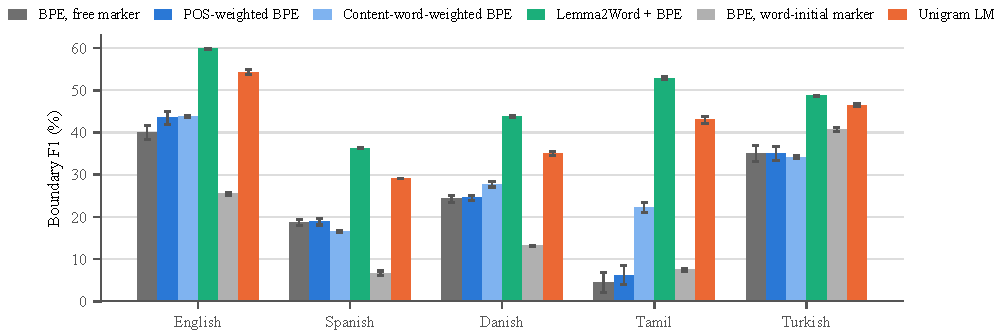
\includegraphics[width=\linewidth]{figures/fig_f1.pdf}
\caption{Boundary F1 (\%) of the six main tokenizers in five languages. Bars are means over three training seeds and error bars span one standard deviation.}
\label{fig:f1}
\end{figure}

Lemma2Word has the highest F1 in every language, from \nFLtwSpanish\% in Spanish to \nFLtwEnglish\% in English.
The unigram model is second everywhere, and ahead of every BPE variant by a wide margin in Tamil (\nFUniTamil\% against \nFBpeTamil\% for free-marker BPE).
The POS-weighted BPE differs from its unweighted base by about three points in English (\nFPosEnglish\% against \nFBpeEnglish\%) and by less than one point in Spanish, Danish and Turkish; only the English difference exceeds the seed-to-seed standard deviation.
Its two ablations show that the transition term carries the whole effect, since \emph{transitions only} reproduces the full variant to the first decimal and \emph{penalty only} is indistinguishable from the unweighted base.
The content-word weighting raises F1 from \nFBpeTamil\% to \nFPosContentTamil\% in Tamil and by about three points in English and Danish, and lowers it in Spanish and Turkish.
The BPE with a word-initial marker, the convention of SentencePiece, has the lowest F1 in four languages; with the whole word and its marker available as a single token, it places fewer boundaries inside words than the free-marker variant (recall \nRHfBpeSpanish\% against \nRBpeSpanish\% in Spanish).

\begin{figure}[!ht]
\centering
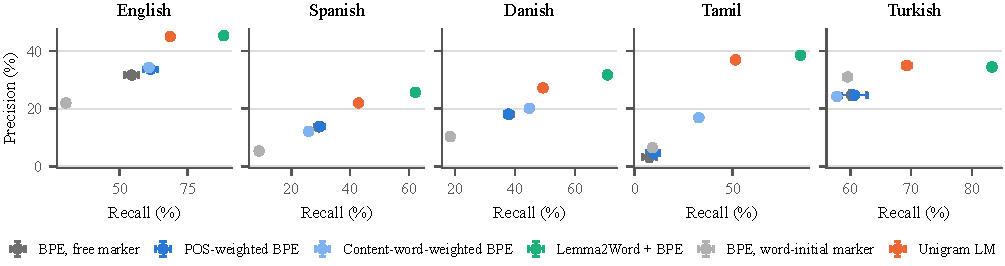
\includegraphics[width=\linewidth]{figures/fig_pr.pdf}
\caption{Boundary precision against recall per language. Points are means over three seeds and error bars span one standard deviation; most are smaller than the markers.}
\label{fig:pr}
\end{figure}

\subsection{What the Part-of-Speech Weighting Changes}\label{sec:res-pos}
The weighting of Section~\ref{sec:posbpe} only changes the score of merges that attach a word to the space after it.
Table~\ref{tab:span} shows what those merges produce on held-out text.
Between \nSpanShareBpeTurkish\% (Turkish) and \nSpanShareBpeSpanish\% (Spanish) of word boundaries end up inside a token under plain free-marker BPE, and the POS weighting leaves those shares almost unchanged except in Tamil, where it lowers the share from \nSpanShareBpeTamil\% to \nSpanSharePosTamil\%\footnote{Seed 0; the three-seed mean of the share of tokens that span a boundary falls from \nCrossBpeTamil\% to \nCrossPosTamil\% (Table~\ref{tab:cross}).}.
The transitions spanned are the ones BPE spans anyway: adposition followed by determiner in English (\texttt{of\textvisiblespace the\textvisiblespace}), determiner followed by noun in Spanish, noun followed by adposition in Danish.
The mean probability of the transition at a spanned boundary is within two points of the mean over all boundaries for every language and every variant, with or without the weighting.
Frequency decides which boundaries a token crosses, and the transition probabilities, which are themselves frequencies of tag pairs, add nothing that the symbol counts do not already contain.

\begin{table}[!ht]
\centering
\caption{Word boundaries spanned by a token on held-out text: share of boundaries (\%), mean probability (\%) of the POS transition at spanned boundaries, and the same mean over all boundaries. Seed 0; the most frequent spanned transition and token are shown for the POS-weighted model.}
\label{tab:span}
\footnotesize
\setlength{\tabcolsep}{3.5pt}
\begin{tabular}{llccclc}
\toprule
Language & System & spanned (\%) & $P$, spanned & $P$, all & top transition & top token \\
\midrule
English & BPE, free marker & 45.2 & 23.3 & 22.1 & ADP$\to$DET & \texttt{in\textvisiblespace{}the\textvisiblespace{}} \\
 & POS-weighted BPE & 42.6 & 23.5 & 22.1 & ADP$\to$DET & \texttt{of\textvisiblespace{}the\textvisiblespace{}} \\
 & Content-word-weighted BPE & 33.2 & 24.4 & 22.1 & ADP$\to$DET & \texttt{of\textvisiblespace{}the\textvisiblespace{}} \\
\addlinespace[2pt]
Spanish & BPE, free marker & 54.1 & 32.3 & 28.2 & DET$\to$NOUN & \texttt{a\textvisiblespace{}de\textvisiblespace{}} \\
 & POS-weighted BPE & 54.1 & 32.3 & 28.2 & DET$\to$NOUN & \texttt{a\textvisiblespace{}de\textvisiblespace{}} \\
 & Content-word-weighted BPE & 43.5 & 33.8 & 28.2 & DET$\to$NOUN & \texttt{en\textvisiblespace{}la\textvisiblespace{}} \\
\addlinespace[2pt]
Danish & BPE, free marker & 41.3 & 21.1 & 22.4 & NOUN$\to$ADP & \texttt{en\textvisiblespace{}i\textvisiblespace{}} \\
 & POS-weighted BPE & 41.4 & 21.1 & 22.4 & NOUN$\to$ADP & \texttt{en\textvisiblespace{}i\textvisiblespace{}} \\
 & Content-word-weighted BPE & 31.0 & 20.9 & 22.4 & NOUN$\to$ADP & \texttt{er\textvisiblespace{}i\textvisiblespace{}} \\
\addlinespace[2pt]
Tamil & BPE, free marker & 54.1 & 24.4 & 24.9 & NOUN$\to$NOUN & \tamil{ு}\textvisiblespace{}\tamil{ப} \\
 & POS-weighted BPE & 39.5 & 25.0 & 24.9 & NOUN$\to$NOUN & \tamil{ு}\textvisiblespace{}\tamil{ப} \\
 & Content-word-weighted BPE & 7.4 & 26.5 & 24.9 & NOUN$\to$NOUN & \tamil{ப்}\textvisiblespace{}\tamil{ப} \\
\addlinespace[2pt]
Turkish & BPE, free marker & 15.5 & 22.3 & 25.0 & NOUN$\to$CCONJ & \texttt{i\textvisiblespace{}ve\textvisiblespace{}} \\
 & POS-weighted BPE & 15.2 & 22.5 & 25.0 & NOUN$\to$CCONJ & \texttt{i\textvisiblespace{}ve\textvisiblespace{}} \\
 & Content-word-weighted BPE & 9.0 & 23.7 & 25.0 & NOUN$\to$CCONJ & \texttt{i\textvisiblespace{}ve\textvisiblespace{}} \\
\addlinespace[2pt]
\bottomrule
\end{tabular}
\end{table}


\subsection{Content-Word Weighting}\label{sec:res-content}
Doubling the weight of merges inside nouns, proper nouns, verbs and adjectives has the effect it was designed to have, a vocabulary that spends more of its budget on whole content words, and that effect helps or hurts depending on the language.
It lowers the share of tokens that span a word boundary everywhere (Table~\ref{tab:cross}) and raises recall in Tamil from \nRBpeTamil\% to \nRPosContentTamil\%, where plain BPE almost never cuts at the stem boundary.
In Spanish and Turkish it lowers recall, because the whole-word tokens it buys replace the suffix tokens that plain BPE learns there.
The weight of 2 was fixed in advance; a sweep over it would turn the variant into a tuned method and was not run.

\subsection{Lemma2Word}\label{sec:res-l2w}
Table~\ref{tab:l2w} separates the lexicon variant, which uses nothing beyond what it learned from the training text, from the online variant, which lemmatizes every evaluation word with Stanza, and reports both on all forms, on forms absent from the training text, and on forms from the Universal Dependencies test split.

\begin{table}[!ht]
\centering
\caption{Lemma2Word boundary recall and precision (\%) by word subset: all unique forms, forms absent from the tokenizer's training text, and forms from the UD test split. \emph{Lexicon} uses only boundaries and affixes learned from the training text; \emph{online} also lemmatizes the evaluation word with Stanza at tokenization time. Mean over three seeds.}
\label{tab:l2w}
\small
\setlength{\tabcolsep}{3.5pt}
\begin{tabular}{llcccccc}
\toprule
 & & \multicolumn{2}{c}{all} & \multicolumn{2}{c}{unseen} & \multicolumn{2}{c}{UD test} \\
\cmidrule(lr){3-4}\cmidrule(lr){5-6}\cmidrule(lr){7-8}
Language & Variant & R & P & R & P & R & P \\
\midrule
English & lexicon & 88.2 & 45.3 & 73.7 & 30.3 & 84.0 & 37.2 \\
 & online & 98.2 & 50.9 & 98.2 & 41.1 & 91.1 & 40.9 \\
 & BPE, free marker & 54.4 & 31.6 & 54.5 & 25.5 & 49.2 & 24.8 \\
\addlinespace[2pt]
Spanish & lexicon & 62.2 & 25.6 & 40.2 & 15.3 & 48.1 & 18.3 \\
 & online & 99.1 & 39.0 & 99.1 & 35.4 & 94.8 & 34.2 \\
 & BPE, free marker & 29.4 & 13.7 & 35.8 & 14.7 & 31.8 & 13.2 \\
\addlinespace[2pt]
Danish & lexicon & 70.8 & 31.7 & 49.5 & 17.9 & 65.5 & 27.2 \\
 & online & 97.2 & 43.6 & 97.1 & 35.3 & 88.0 & 37.0 \\
 & BPE, free marker & 37.9 & 17.9 & 41.0 & 15.9 & 38.0 & 16.7 \\
\addlinespace[2pt]
Tamil & lexicon & 84.5 & 38.5 & 74.2 & 27.4 & 80.6 & 34.7 \\
 & online & 97.6 & 46.3 & 97.7 & 38.5 & 91.5 & 39.9 \\
 & BPE, free marker & 7.4 & 3.2 & 7.0 & 2.5 & 5.9 & 2.4 \\
\addlinespace[2pt]
Turkish & lexicon & 83.3 & 34.4 & 81.7 & 31.2 & 82.7 & 32.0 \\
 & online & 88.6 & 37.6 & 88.4 & 34.8 & 89.1 & 35.6 \\
 & BPE, free marker & 60.2 & 24.7 & 60.5 & 23.2 & 60.4 & 23.2 \\
\addlinespace[2pt]
\bottomrule
\end{tabular}
\end{table}


On all forms, the lexicon variant raises recall over free-marker BPE from \nRBpeEnglish\% to \nLtwLexiconAllREnglish\% in English, from \nRBpeTamil\% to \nLtwLexiconAllRTamil\% in Tamil, and by 23 to 34 points in the other three languages, while precision rises as well, since the pieces it hands to BPE are shorter and BPE places fewer boundaries inside them.
On unseen forms, where only the affix inventories can act, recall is \nLtwLexiconUnseenREnglish\% in English and \nLtwLexiconUnseenRTamil\% in Tamil, and it shrinks to a few points in Spanish and Danish, whose inflectional suffixes are short and ambiguous with word-final letter sequences, so that the 20-occurrence threshold admits few of them.
The online variant recovers almost every gold boundary (\nLtwOnlineAllRSpanish\% recall in Spanish), which is expected, because the gold boundaries are themselves derived from lemmas and, on forms from the treebank training split, the lemmatizer can return the gold lemma from memory.
On the test-split forms, which the lemmatizer never saw, recall is lower but still between \nLtwOnlineTestRDanish\% and \nLtwOnlineTestRSpanish\%.
The precision of the online variant stays below 51\% because BPE goes on splitting inside the pieces; the gold standard records only the stem boundary.

\subsection{Compression and Stability}\label{sec:res-compression}
Table~\ref{tab:tpw} reports tokens per word on held-out text.
The POS weighting changes compression by less than one percent.
Lemma2Word needs \nTpwLtwEnglish{} tokens per word in English against \nTpwBpeEnglish{} for free-marker BPE (four percent more) and \nTpwLtwSpanish{} against \nTpwBpeSpanish{} in Spanish (eight percent more), and it is still more compact than the unigram model in every language but Tamil.
The two reference tokenizers, which never cross a word boundary, need more tokens per word than free-marker BPE in the three European languages and fewer in Tamil and Turkish, where free-marker BPE spends part of its budget on tokens that span frequent word pairs.

\begin{table}[!ht]
\centering
\caption{Tokens per whitespace word on held-out Wikipedia paragraphs (lower is more compact).}
\label{tab:tpw}
\small
\setlength{\tabcolsep}{4pt}
\begin{tabular}{lccccc}
\toprule
System & English & Spanish & Danish & Tamil & Turkish \\
\midrule
BPE, free marker & 1.481\,{\scriptsize$\pm$0.002} & 1.413\,{\scriptsize$\pm$0.002} & 1.606\,{\scriptsize$\pm$0.002} & 2.242\,{\scriptsize$\pm$0.005} & 1.962\,{\scriptsize$\pm$0.002} \\
POS-weighted BPE & 1.470\,{\scriptsize$\pm$0.001} & \textbf{1.412\,{\scriptsize$\pm$0.001}} & \textbf{1.604\,{\scriptsize$\pm$0.002}} & 2.215\,{\scriptsize$\pm$0.006} & 1.938\,{\scriptsize$\pm$0.025} \\
\quad transitions only & 1.470\,{\scriptsize$\pm$0.001} & 1.412\,{\scriptsize$\pm$0.001} & 1.604\,{\scriptsize$\pm$0.002} & 2.215\,{\scriptsize$\pm$0.006} & 1.938\,{\scriptsize$\pm$0.025} \\
\quad penalty only & \textbf{1.470\,{\scriptsize$\pm$0.001}} & 1.413\,{\scriptsize$\pm$0.002} & 1.605\,{\scriptsize$\pm$0.002} & 2.243\,{\scriptsize$\pm$0.005} & 1.962\,{\scriptsize$\pm$0.003} \\
\addlinespace[2pt]
Content-word-weighted BPE & 1.486\,{\scriptsize$\pm$0.002} & 1.423\,{\scriptsize$\pm$0.002} & 1.619\,{\scriptsize$\pm$0.001} & 2.150\,{\scriptsize$\pm$0.012} & 1.998\,{\scriptsize$\pm$0.003} \\
Lemma2Word + BPE & 1.538\,{\scriptsize$\pm$0.001} & 1.531\,{\scriptsize$\pm$0.002} & 1.703\,{\scriptsize$\pm$0.001} & 2.376\,{\scriptsize$\pm$0.002} & 2.080\,{\scriptsize$\pm$0.010} \\
BPE, word-initial marker & 1.555\,{\scriptsize$\pm$0.001} & 1.565\,{\scriptsize$\pm$0.000} & 1.713\,{\scriptsize$\pm$0.001} & \textbf{2.042\,{\scriptsize$\pm$0.001}} & \textbf{1.883\,{\scriptsize$\pm$0.002}} \\
Unigram LM & 1.609\,{\scriptsize$\pm$0.001} & 1.607\,{\scriptsize$\pm$0.002} & 1.778\,{\scriptsize$\pm$0.004} & 2.177\,{\scriptsize$\pm$0.006} & 2.004\,{\scriptsize$\pm$0.004} \\
\bottomrule
\end{tabular}
\end{table}


Stability across training samples (Tables~\ref{tab:jaccard} and~\ref{tab:agreement} in the appendix) separates the methods less than accuracy does.
Two vocabularies learned from different samples share between 62\% and 79\% of their entries by the Jaccard measure, and two tokenizers of the same method segment the same held-out text with a boundary agreement of 88\% to 97\%.
The POS weighting does not improve either number; in Turkish it lowers vocabulary overlap from \nJacBpeTurkish\% to \nJacPosTurkish\% with a standard deviation of \nJacPosTurkishSd{} points, the least stable entry in the table.
The unigram model has the lowest vocabulary overlap in every language and an agreement comparable to the others, so its vocabularies vary in the rare entries that seldom appear in held-out text.

\subsection{Vocabulary Budget}\label{sec:res-sweep}
Figure~\ref{fig:sweep} repeats the comparison at budgets of 2,000 and 32,000 types with seed 0.
The ordering of the methods is the same at every budget.
Lemma2Word gains with the budget in every language, from \nSweepFLtwEnglishVTwoK\% to \nSweepFLtwEnglishVThirtyTwoK\% in English, because a larger vocabulary leaves its pieces whole more often.
The unigram model loses accuracy at 32,000 types in English, Tamil and Turkish, where that budget exceeds the number of word types a 3,000-paragraph sample can support and whole words enter the vocabulary.
The gap between the POS-weighted and the unweighted BPE stays within three points at every budget.

\begin{figure}[!ht]
\centering
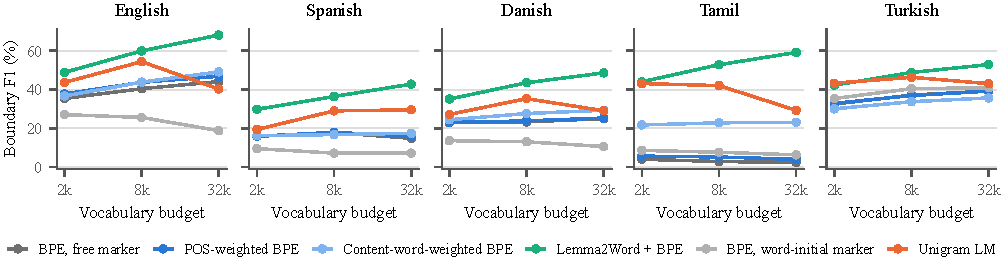
\includegraphics[width=\linewidth]{figures/fig_sweep.pdf}
\caption{Boundary F1 (\%) at vocabulary budgets of 2,000, 8,000 and 32,000 types, seed 0.}
\label{fig:sweep}
\end{figure}

\subsection{Language-Model Probe}\label{sec:res-lm}
Table~\ref{tab:bpc} and Figure~\ref{fig:bpc} report the bits per character of the language model trained on each tokenizer's output, with one model per tokenizer seed.
The seed-to-seed standard deviation is below 0.01 bits for most entries and 0.03 at worst, so differences of a few hundredths are reliable at this scale.

\begin{table}[!ht]
\centering
\caption{Bits per character of a 7M-parameter language model trained for six passes over the same text with each tokenizer (lower is better). Mean $\pm$ standard deviation over the three tokenizer seeds.}
\label{tab:bpc}
\small
\setlength{\tabcolsep}{4pt}
\begin{tabular}{lccccc}
\toprule
System & English & Spanish & Danish & Tamil & Turkish \\
\midrule
BPE, free marker & 2.807\,{\scriptsize$\pm$0.002} & 2.689\,{\scriptsize$\pm$0.003} & 2.878\,{\scriptsize$\pm$0.001} & 2.848\,{\scriptsize$\pm$0.006} & 2.963\,{\scriptsize$\pm$0.002} \\
POS-weighted BPE & 2.785\,{\scriptsize$\pm$0.001} & 2.687\,{\scriptsize$\pm$0.001} & 2.874\,{\scriptsize$\pm$0.001} & 2.819\,{\scriptsize$\pm$0.005} & 2.935\,{\scriptsize$\pm$0.032} \\
\quad transitions only & 2.785\,{\scriptsize$\pm$0.001} & 2.687\,{\scriptsize$\pm$0.001} & 2.874\,{\scriptsize$\pm$0.002} & 2.819\,{\scriptsize$\pm$0.005} & 2.935\,{\scriptsize$\pm$0.032} \\
\quad penalty only & 2.786\,{\scriptsize$\pm$0.002} & 2.689\,{\scriptsize$\pm$0.002} & 2.876\,{\scriptsize$\pm$0.001} & 2.849\,{\scriptsize$\pm$0.006} & 2.963\,{\scriptsize$\pm$0.003} \\
\addlinespace[2pt]
Content-word-weighted BPE & 2.794\,{\scriptsize$\pm$0.001} & 2.680\,{\scriptsize$\pm$0.003} & 2.868\,{\scriptsize$\pm$0.001} & 2.737\,{\scriptsize$\pm$0.015} & 2.995\,{\scriptsize$\pm$0.003} \\
Lemma2Word + BPE & 2.887\,{\scriptsize$\pm$0.003} & 2.861\,{\scriptsize$\pm$0.004} & 3.007\,{\scriptsize$\pm$0.001} & 2.983\,{\scriptsize$\pm$0.002} & 3.096\,{\scriptsize$\pm$0.011} \\
BPE, word-initial marker & 2.715\,{\scriptsize$\pm$0.003} & 2.674\,{\scriptsize$\pm$0.006} & 2.909\,{\scriptsize$\pm$0.003} & 2.611\,{\scriptsize$\pm$0.001} & 2.808\,{\scriptsize$\pm$0.004} \\
Unigram LM & \textbf{2.531\,{\scriptsize$\pm$0.006}} & \textbf{2.473\,{\scriptsize$\pm$0.011}} & \textbf{2.704\,{\scriptsize$\pm$0.007}} & \textbf{2.524\,{\scriptsize$\pm$0.003}} & \textbf{2.694\,{\scriptsize$\pm$0.003}} \\
\bottomrule
\end{tabular}
\end{table}


\begin{figure}[!ht]
\centering
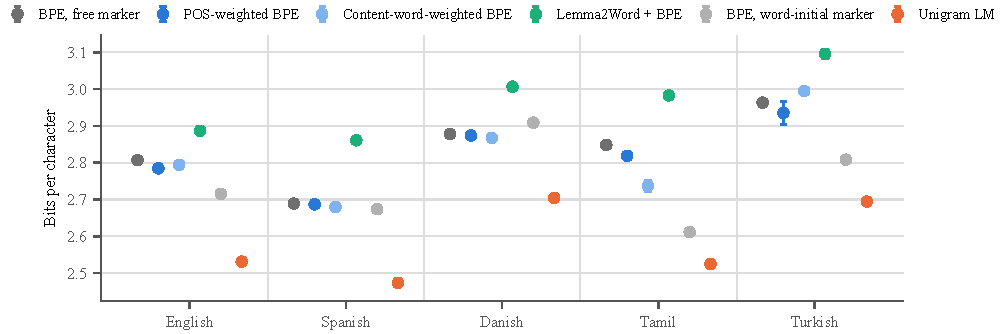
\includegraphics[width=\linewidth]{figures/fig_bpc.pdf}
\caption{Bits per character of a 7M-parameter language model trained for six passes over the same text with each tokenizer (lower is better). Points are means over the three tokenizer seeds and error bars span one standard deviation; the vertical axis starts at 2.4 bits so that the differences are visible.}
\label{fig:bpc}
\end{figure}

The ordering by bits per character is not the ordering by boundary F1.
The unigram model, second by F1, is first by a wide margin in every language, at \nBpcUniEnglish{} bits against \nBpcBpeEnglish{} for free-marker BPE in English and \nBpcUniTamil{} against \nBpcBpeTamil{} in Tamil.
Lemma2Word, first by F1 everywhere, is last by bits per character everywhere (\nBpcLtwEnglish{} in English).
Cutting words at the stem boundary before subword training removes frequent whole-word tokens from the vocabulary, and the extra tokens it produces are not predictable enough, for a model of this size, to pay for themselves.
The word-initial-marker BPE, last by F1 in four languages, is better than free-marker BPE by bits per character in four languages (\nBpcHfBpeEnglish{} against \nBpcBpeEnglish{} in English); the tokens that span word boundaries, which make the free-marker variant more compact, do not help prediction.
The POS weighting changes bits per character by less than 0.03 in every language, in the direction of a small improvement, with the largest seed-to-seed variation of the table in Turkish, and its two ablations again coincide with it.
The content-word weighting lowers bits per character in Tamil (\nBpcPosContentTamil{} against \nBpcBpeTamil), where it also raised boundary F1 most, and raises them in Turkish.

Because every model is trained for six passes over the same text, a tokenizer that produces more tokens also gives its model more optimizer steps, 8.6\% more for the unigram model than for free-marker BPE in English.
A control that trains the free-marker BPE model of seed 0 for 5.4 and 6.6 passes, 10\% fewer and 10\% more steps, moves its bits per character from \nBpcControlBase{} to \nBpcControlLow{} and \nBpcControlHigh{}, far less than the gaps between tokenizers, and Lemma2Word produces more tokens than free-marker BPE yet scores worse, so the step count does not explain the ordering.
What the probe shows is that morphological alignment and modeling quality do not move together at this scale, in agreement with \citet{bostrom2020bpe} on the unigram model and with the broader finding that intrinsic tokenizer measures predict downstream quality imperfectly~\cite{schmidt2024tokenization,ali2024tokenizer}.

\subsection{A Language Model as a Segmenter}\label{sec:res-llm}
Table~\ref{tab:llm} reports the segmentation study of Section~\ref{sec:llm}.
For each language, 400 word forms were drawn at random (seed 0) from the gold list, and Claude Sonnet (model string \texttt{claude-sonnet-5-5}, October 2026) was asked, in batches of 40 words, to insert plus signs at the morpheme boundaries without changing a character; the prompt is given in Appendix~\ref{app:prompt}.
An answer whose characters differ from the word is invalid and is excluded from the scores.
To compare like with like, the seed-0 tokenizers are scored on exactly the words the model answered validly.

\begin{table}[!ht]
\centering
\caption{A language model (Claude Sonnet) prompted to segment words into morphemes, scored on a fixed random sample of the gold word forms, beside three tokenizers (seed 0) scored on the same words. \emph{Invalid}: answers that changed the characters of the word and were excluded. Boundary precision, recall and F1 in \%; tokens per word is the number of pieces.}
\label{tab:llm}
\small
\setlength{\tabcolsep}{3.5pt}
\begin{tabular}{lrrcccccccc}
\toprule
 & & & \multicolumn{4}{c}{language model} & \multicolumn{3}{c}{recall of tokenizers on the same words} \\
\cmidrule(lr){4-7}\cmidrule(lr){8-10}
Language & words & invalid & P & R & F1 & pieces/word & Lemma2Word & Unigram & BPE, free \\
\midrule
English & 400 & 0 & 77.6 & 91.0 & 83.8 & 2.17 & 87.0 & 69.2 & 52.2 \\
Spanish & 399 & 1 & 35.1 & 69.9 & 46.8 & 2.99 & 62.2 & 44.1 & 25.3 \\
Danish & 400 & 0 & 38.9 & 66.0 & 49.0 & 2.69 & 72.5 & 50.0 & 42.0 \\
Tamil & 393 & 7 & 72.6 & 90.4 & 80.5 & 2.25 & 84.8 & 48.9 & 6.8 \\
Turkish & 400 & 0 & 50.7 & 96.5 & 66.5 & 2.90 & 84.8 & 67.2 & 60.2 \\
\bottomrule
\end{tabular}
\end{table}


The model recovers more gold boundaries than any tokenizer in four languages, with \nLlmREnglish\% recall in English against \nLlmSampleLtwREnglish\% for Lemma2Word on the same words, \nLlmRTamil\% against \nLlmSampleLtwRTamil\% in Tamil and \nLlmRTurkish\% against \nLlmSampleLtwRTurkish\% in Turkish, and it trails Lemma2Word in Danish (\nLlmRDanish\% against \nLlmSampleLtwRDanish\%).
Its precision is between \nLlmPSpanish\% and \nLlmPEnglish\%, because it marks derivational affixes and compound parts that the lemma-derived gold standard does not, producing \nLlmTpwEnglish{} to \nLlmTpwSpanish{} pieces per word where the gold has at most three.
Almost every answer preserved the characters in the four Latin-script languages (\nLlmInvalidSpanish{} invalid answer in Spanish, none elsewhere).
Tamil was harder in two ways.
The model reasoned at length before answering, so that 40-word batches overran the reply length and the unanswered words had to be re-asked in batches of 15, and \nLlmInvalidTamil{} answers wrote the underlying morphemes instead of the surface string (\tamil{கள்}\,+\,\tamil{உக்கு} for \tamil{களுக்கு}, where the vowel of the suffix fuses with the preceding consonant in writing), which the character constraint forbids.
The study used about 2,000 words and a few dollars of API usage, and it shows what the model knows about morphology rather than what a tokenizer built from it would do: the answers have no fixed vocabulary, are not guaranteed to be consistent across occurrences of a word, and cost several orders of magnitude more per word than any tokenizer in Table~\ref{tab:f1}.
Used offline, to write a segmentation lexicon in the manner of Lemma2Word's, such answers could supply boundaries where no lemmatizer exists; that use is not evaluated here.


\section{Discussion}\label{sec:discussion}

\paragraph{Why the transition weighting cannot work.}
A merge score in BPE is a count of adjacent symbol pairs, and the POS-weighted variant multiplies the count of a pair at a word boundary by one plus the probability of the tag transition there.
Since that probability is a function of the two words' tags and the tags are a function of the words, the weight is a smoothed version of the pair's own frequency, so that \emph{of the} is merged because it is frequent and the weighting adds a bonus for the same reason.
Table~\ref{tab:span} shows the consequence, with the same tokens crossing word boundaries with and without the weighting and a transition probability at a spanned boundary no higher than at an unspanned one.
A signal about the order of words cannot say where to cut inside a word, which is where the gold boundaries lie, and the design never gave it a way to.

\paragraph{What the preliminary diagnostics measured.}
The earlier report described lower segmentation entropy, longer tokens, gains of 12 to 20 points in a transition-accuracy diagnostic and of about 20 points in vocabulary reuse.
None of those quantities was computed against held-out words or a gold standard, and the implementation they came from scored transitions against the wrong words after its first space-absorbing merge (Section~\ref{sec:posbpe}).
Under the protocol of Section~\ref{sec:protocol} vocabulary reuse does not change (Table~\ref{tab:jaccard}), token length changes by less than one percent (Table~\ref{tab:tpw}), and the only method with a consistent effect on morphological boundaries is the one that uses a lemmatizer.

\paragraph{Lemmas against tags.}
A lemma says where a word's stem ends, whereas a tag says what kind of word it is, and only the first is information about boundaries, from which the results follow.
Lemma2Word moves recall by 23 to 77 points, and the part of that gain which survives on unseen words depends on how far an affix inventory generalizes, well for English and Turkish, where the suffixes are long and distinctive, and poorly for Spanish and Danish, where they are short.
The online variant generalizes through the lemmatizer instead and reaches recall of 88\% to 95\% on treebank test forms, at the price of running a neural lemmatizer at tokenization time and of sharing its training data with the gold standard.
The content-word weighting sits between the two, since it uses tags but uses them to decide which words to keep whole, a decision about boundaries, and it helps where whole content words are what the budget was missing, as in Tamil, and hurts where the budget was better spent on suffixes, as in Spanish and Turkish.

\paragraph{Alignment against modeling.}
The probe of Section~\ref{sec:res-lm} separates two things that the literature on morphology-aware tokenization often treats as one.
Finding more gold boundaries did not make a tokenizer better for the language model. The tokenizer that found the most, Lemma2Word, made it worst, and the unigram model, which finds fewer boundaries than Lemma2Word but segments by a probabilistic model of the text, made it best by a margin of a quarter of a bit per character.
The probe is small, and a larger model with more text may close or reverse some of these gaps, but the direction of the result agrees with \citet{bostrom2020bpe} and with the finding that intrinsic measures of a tokenizer predict downstream quality imperfectly~\cite{schmidt2024tokenization,ali2024tokenizer}, and it means that a morphological boundary score alone is not a sufficient reason to adopt a tokenizer.

\paragraph{The marker convention.}
A side result concerns a choice that is rarely discussed, the treatment of the space marker.
Letting it merge freely, as the original implementation does, produces tokens that cross word boundaries at 4\% to 22\% of boundaries and raises boundary F1 over the word-initial-marker convention in four languages, because whole words with a prefixed marker are no longer available as single tokens and the budget goes to pieces instead, while the probe prefers the word-initial convention in the same four languages.
The convention therefore matters as much as any of the linguistic signals tested, and comparisons between tokenizers should hold it fixed.

\paragraph{Limitations.}
The gold standard records at most two boundaries per word, the ones around the stem, so derivational structure inside the stem counts against precision, which makes recall the safer number, although the ranking of the methods is the same under both.
The training samples are small, 3,000 paragraphs per language, because the free-marker implementation is pure Python, and while the vocabulary sweep shows the same ordering at every budget, larger corpora could change the absolute numbers.
Tags and lemmas come from one tagger, the Tamil treebank behind both the tagger and the gold standard is the smallest of the five, and the language-model probe is a 7M-parameter model trained for minutes, which can show that tokenizers differ at that scale but not that they differ at the scale of a large language model.

\section{Conclusion}\label{sec:conclusion}
Part-of-speech tags and lemmas were put into a subword tokenizer in several forms and measured under one protocol in five languages, with gold morpheme boundaries, held-out text, repeated training samples and a language-model probe.
Weighting BPE merges by part-of-speech transitions, the method the authors first proposed, changes neither the boundaries a tokenizer finds nor the text it produces, because a transition probability describes the order of words and not their inside, and weighting merges inside content words changes the vocabulary in the intended direction with an effect on accuracy that depends on the language.
Deriving boundaries from lemmas raises boundary recall substantially everywhere at a cost of four to eight percent more tokens, with a gain on unseen words that depends on how distinctive the affixes of the language are, so a tokenizer that wants morphological boundaries should obtain them from a lemmatizer or a segmentation lexicon, and a tagger adds nothing on top.
What those boundaries are worth to a language model is a separate matter, since the probe ranks the tokenizers in a different order from the boundary scores, with the unigram model first and Lemma2Word last in every language, and the two orders will have to be reconciled at a larger scale than a 7M-parameter model before morphological alignment can be recommended as a design goal.


\paragraph{Author contributions.}
% DRAFT -- all authors must agree on this text before posting.
A.C., J.D.\ and M.V.\ designed the part-of-speech-weighted tokenizer, Lemma2Word and the language-model segmentation study and wrote the original report.
J.D.\ carried out the work reported here: the reimplementation and its corrections, the evaluation protocol, the experiments, and the writing.
% TODO: describe each author's part of the original implementation.


\bibliographystyle{plainnat}
\bibliography{refs}

\appendix
\section{Precision, Recall and Stability by Language}\label{app:tables}
\begin{table}[!ht]
\centering
\caption{Boundary precision (\%).}
\label{tab:precision}
\small
\setlength{\tabcolsep}{4pt}
\begin{tabular}{lccccc}
\toprule
System & English & Spanish & Danish & Tamil & Turkish \\
\midrule
BPE, free marker & 31.6\,{\scriptsize$\pm$1.2} & 13.7\,{\scriptsize$\pm$0.5} & 17.9\,{\scriptsize$\pm$0.6} & 3.2\,{\scriptsize$\pm$1.7} & 24.7\,{\scriptsize$\pm$1.4} \\
POS-weighted BPE & 33.6\,{\scriptsize$\pm$1.1} & 13.8\,{\scriptsize$\pm$0.6} & 18.1\,{\scriptsize$\pm$0.3} & 4.5\,{\scriptsize$\pm$1.7} & 24.6\,{\scriptsize$\pm$1.3} \\
\quad transitions only & 33.6\,{\scriptsize$\pm$1.2} & 13.8\,{\scriptsize$\pm$0.6} & 18.1\,{\scriptsize$\pm$0.3} & 4.6\,{\scriptsize$\pm$1.7} & 24.6\,{\scriptsize$\pm$1.3} \\
\quad penalty only & 32.7\,{\scriptsize$\pm$0.9} & 13.7\,{\scriptsize$\pm$0.5} & 18.0\,{\scriptsize$\pm$0.7} & 3.2\,{\scriptsize$\pm$1.7} & 24.6\,{\scriptsize$\pm$1.5} \\
\addlinespace[2pt]
Content-word-weighted BPE & 34.3\,{\scriptsize$\pm$0.2} & 12.1\,{\scriptsize$\pm$0.2} & 20.1\,{\scriptsize$\pm$0.5} & 16.8\,{\scriptsize$\pm$0.9} & 24.2\,{\scriptsize$\pm$0.3} \\
Lemma2Word + BPE & \textbf{45.3\,{\scriptsize$\pm$0.1}} & \textbf{25.6\,{\scriptsize$\pm$0.1}} & \textbf{31.7\,{\scriptsize$\pm$0.2}} & \textbf{38.5\,{\scriptsize$\pm$0.4}} & 34.4\,{\scriptsize$\pm$0.1} \\
BPE, word-initial marker & 22.0\,{\scriptsize$\pm$0.3} & 5.3\,{\scriptsize$\pm$0.4} & 10.2\,{\scriptsize$\pm$0.1} & 6.4\,{\scriptsize$\pm$0.3} & 31.0\,{\scriptsize$\pm$0.3} \\
Unigram LM & 45.0\,{\scriptsize$\pm$0.5} & 21.9\,{\scriptsize$\pm$0.0} & 27.2\,{\scriptsize$\pm$0.4} & 36.9\,{\scriptsize$\pm$0.8} & \textbf{35.0\,{\scriptsize$\pm$0.3}} \\
\bottomrule
\end{tabular}
\end{table}

\begin{table}[!ht]
\centering
\caption{Boundary recall (\%).}
\label{tab:recall}
\small
\setlength{\tabcolsep}{4pt}
\begin{tabular}{lccccc}
\toprule
System & English & Spanish & Danish & Tamil & Turkish \\
\midrule
BPE, free marker & 54.4\,{\scriptsize$\pm$2.6} & 29.4\,{\scriptsize$\pm$1.5} & 37.9\,{\scriptsize$\pm$1.5} & 7.4\,{\scriptsize$\pm$3.7} & 60.2\,{\scriptsize$\pm$2.4} \\
POS-weighted BPE & 61.3\,{\scriptsize$\pm$2.5} & 29.8\,{\scriptsize$\pm$1.5} & 37.9\,{\scriptsize$\pm$1.3} & 9.5\,{\scriptsize$\pm$3.3} & 60.7\,{\scriptsize$\pm$2.1} \\
\quad transitions only & 61.3\,{\scriptsize$\pm$2.5} & 29.8\,{\scriptsize$\pm$1.5} & 37.9\,{\scriptsize$\pm$1.3} & 9.6\,{\scriptsize$\pm$3.3} & 60.7\,{\scriptsize$\pm$2.1} \\
\quad penalty only & 58.7\,{\scriptsize$\pm$2.0} & 29.4\,{\scriptsize$\pm$1.5} & 37.9\,{\scriptsize$\pm$1.6} & 7.4\,{\scriptsize$\pm$3.7} & 60.1\,{\scriptsize$\pm$2.5} \\
\addlinespace[2pt]
Content-word-weighted BPE & 60.8\,{\scriptsize$\pm$0.3} & 25.9\,{\scriptsize$\pm$0.5} & 44.8\,{\scriptsize$\pm$1.1} & 32.7\,{\scriptsize$\pm$1.6} & 57.8\,{\scriptsize$\pm$0.4} \\
Lemma2Word + BPE & \textbf{88.2\,{\scriptsize$\pm$0.1}} & \textbf{62.2\,{\scriptsize$\pm$0.3}} & \textbf{70.8\,{\scriptsize$\pm$0.5}} & \textbf{84.5\,{\scriptsize$\pm$0.5}} & \textbf{83.3\,{\scriptsize$\pm$0.3}} \\
BPE, word-initial marker & 30.3\,{\scriptsize$\pm$0.4} & 9.1\,{\scriptsize$\pm$0.7} & 18.4\,{\scriptsize$\pm$0.2} & 9.0\,{\scriptsize$\pm$0.4} & 59.6\,{\scriptsize$\pm$0.7} \\
Unigram LM & 68.6\,{\scriptsize$\pm$0.4} & 42.9\,{\scriptsize$\pm$0.2} & 49.3\,{\scriptsize$\pm$0.6} & 51.5\,{\scriptsize$\pm$0.9} & 69.3\,{\scriptsize$\pm$0.7} \\
\bottomrule
\end{tabular}
\end{table}

\begin{table}[!ht]
\centering
\caption{Share of held-out tokens that span a word boundary (\%).}
\label{tab:cross}
\small
\setlength{\tabcolsep}{4pt}
\begin{tabular}{lccccc}
\toprule
System & English & Spanish & Danish & Tamil & Turkish \\
\midrule
BPE, free marker & 15.2\,{\scriptsize$\pm$0.1} & 18.3\,{\scriptsize$\pm$0.0} & 13.1\,{\scriptsize$\pm$0.1} & \textbf{22.0\,{\scriptsize$\pm$1.5}} & 4.5\,{\scriptsize$\pm$0.1} \\
POS-weighted BPE & 14.2\,{\scriptsize$\pm$0.1} & 18.4\,{\scriptsize$\pm$0.0} & 13.2\,{\scriptsize$\pm$0.2} & 15.6\,{\scriptsize$\pm$2.4} & 4.4\,{\scriptsize$\pm$0.1} \\
\quad transitions only & 14.2\,{\scriptsize$\pm$0.1} & 18.4\,{\scriptsize$\pm$0.0} & 13.2\,{\scriptsize$\pm$0.2} & 15.6\,{\scriptsize$\pm$2.4} & 4.4\,{\scriptsize$\pm$0.1} \\
\quad penalty only & 14.4\,{\scriptsize$\pm$0.0} & 18.3\,{\scriptsize$\pm$0.0} & 13.2\,{\scriptsize$\pm$0.1} & 21.9\,{\scriptsize$\pm$1.5} & 4.5\,{\scriptsize$\pm$0.1} \\
\addlinespace[2pt]
Content-word-weighted BPE & 10.9\,{\scriptsize$\pm$0.2} & 14.5\,{\scriptsize$\pm$0.1} & 9.7\,{\scriptsize$\pm$0.2} & 2.2\,{\scriptsize$\pm$0.3} & 2.5\,{\scriptsize$\pm$0.1} \\
Lemma2Word + BPE & \textbf{15.7\,{\scriptsize$\pm$0.0}} & \textbf{19.2\,{\scriptsize$\pm$0.0}} & \textbf{15.4\,{\scriptsize$\pm$0.1}} & 12.8\,{\scriptsize$\pm$0.2} & \textbf{6.6\,{\scriptsize$\pm$0.1}} \\
BPE, word-initial marker & 0.0\,{\scriptsize$\pm$0.0} & 0.0\,{\scriptsize$\pm$0.0} & 0.0\,{\scriptsize$\pm$0.0} & 0.0\,{\scriptsize$\pm$0.0} & 0.0\,{\scriptsize$\pm$0.0} \\
Unigram LM & 0.0\,{\scriptsize$\pm$0.0} & 0.0\,{\scriptsize$\pm$0.0} & 0.0\,{\scriptsize$\pm$0.0} & 0.0\,{\scriptsize$\pm$0.0} & 0.0\,{\scriptsize$\pm$0.0} \\
\bottomrule
\end{tabular}
\end{table}

\begin{table}[!ht]
\centering
\caption{Vocabulary reuse: Jaccard overlap (\%) between the vocabularies learned from different training samples (three seed pairs).}
\label{tab:jaccard}
\small
\setlength{\tabcolsep}{4pt}
\begin{tabular}{lccccc}
\toprule
System & English & Spanish & Danish & Tamil & Turkish \\
\midrule
BPE, free marker & 76.8\,{\scriptsize$\pm$0.8} & 75.8\,{\scriptsize$\pm$1.8} & 76.8\,{\scriptsize$\pm$0.4} & 63.8\,{\scriptsize$\pm$4.8} & 74.6\,{\scriptsize$\pm$1.9} \\
POS-weighted BPE & 77.8\,{\scriptsize$\pm$0.9} & 76.3\,{\scriptsize$\pm$2.0} & 76.7\,{\scriptsize$\pm$0.6} & 61.9\,{\scriptsize$\pm$5.4} & 67.1\,{\scriptsize$\pm$7.4} \\
\quad transitions only & 77.8\,{\scriptsize$\pm$0.9} & 76.2\,{\scriptsize$\pm$2.0} & 76.6\,{\scriptsize$\pm$0.5} & 61.8\,{\scriptsize$\pm$5.4} & 67.2\,{\scriptsize$\pm$7.4} \\
\quad penalty only & 77.1\,{\scriptsize$\pm$0.7} & 75.8\,{\scriptsize$\pm$1.8} & 76.3\,{\scriptsize$\pm$0.4} & 64.1\,{\scriptsize$\pm$4.8} & 75.1\,{\scriptsize$\pm$2.3} \\
\addlinespace[2pt]
Content-word-weighted BPE & 74.8\,{\scriptsize$\pm$3.1} & \textbf{77.2\,{\scriptsize$\pm$0.3}} & 74.3\,{\scriptsize$\pm$2.4} & 71.5\,{\scriptsize$\pm$2.5} & 77.0\,{\scriptsize$\pm$1.0} \\
Lemma2Word + BPE & 76.9\,{\scriptsize$\pm$0.7} & 75.6\,{\scriptsize$\pm$1.5} & \textbf{77.8\,{\scriptsize$\pm$0.6}} & 74.8\,{\scriptsize$\pm$0.5} & 74.1\,{\scriptsize$\pm$3.1} \\
BPE, word-initial marker & \textbf{78.5\,{\scriptsize$\pm$0.4}} & 74.4\,{\scriptsize$\pm$3.2} & 76.1\,{\scriptsize$\pm$0.9} & \textbf{76.9\,{\scriptsize$\pm$0.2}} & \textbf{78.5\,{\scriptsize$\pm$1.1}} \\
Unigram LM & 69.3\,{\scriptsize$\pm$1.1} & 66.3\,{\scriptsize$\pm$0.7} & 62.7\,{\scriptsize$\pm$0.2} & 62.9\,{\scriptsize$\pm$0.6} & 69.1\,{\scriptsize$\pm$0.4} \\
\bottomrule
\end{tabular}
\end{table}

\begin{table}[!ht]
\centering
\caption{Segmentation agreement: boundary F1 (\%) between the held-out segmentations of tokenizers trained on different samples (three seed pairs).}
\label{tab:agreement}
\small
\setlength{\tabcolsep}{4pt}
\begin{tabular}{lccccc}
\toprule
System & English & Spanish & Danish & Tamil & Turkish \\
\midrule
BPE, free marker & 95.2\,{\scriptsize$\pm$0.1} & 95.1\,{\scriptsize$\pm$0.8} & 95.7\,{\scriptsize$\pm$0.2} & 88.6\,{\scriptsize$\pm$3.4} & 94.6\,{\scriptsize$\pm$1.2} \\
POS-weighted BPE & 95.8\,{\scriptsize$\pm$0.1} & 95.2\,{\scriptsize$\pm$0.9} & 95.5\,{\scriptsize$\pm$0.3} & 87.5\,{\scriptsize$\pm$3.3} & 92.5\,{\scriptsize$\pm$2.7} \\
\quad transitions only & 95.8\,{\scriptsize$\pm$0.1} & 95.3\,{\scriptsize$\pm$0.9} & 95.5\,{\scriptsize$\pm$0.3} & 87.6\,{\scriptsize$\pm$3.4} & 92.5\,{\scriptsize$\pm$2.7} \\
\quad penalty only & 95.6\,{\scriptsize$\pm$0.2} & 95.1\,{\scriptsize$\pm$0.8} & 95.5\,{\scriptsize$\pm$0.1} & 88.7\,{\scriptsize$\pm$3.5} & 94.7\,{\scriptsize$\pm$1.3} \\
\addlinespace[2pt]
Content-word-weighted BPE & 95.0\,{\scriptsize$\pm$1.1} & \textbf{95.9\,{\scriptsize$\pm$0.1}} & 95.5\,{\scriptsize$\pm$0.6} & 94.0\,{\scriptsize$\pm$0.9} & \textbf{96.0\,{\scriptsize$\pm$0.2}} \\
Lemma2Word + BPE & 95.2\,{\scriptsize$\pm$0.3} & 94.9\,{\scriptsize$\pm$0.6} & 95.8\,{\scriptsize$\pm$0.2} & 94.7\,{\scriptsize$\pm$0.2} & 95.6\,{\scriptsize$\pm$0.7} \\
BPE, word-initial marker & \textbf{96.9\,{\scriptsize$\pm$0.1}} & 95.5\,{\scriptsize$\pm$1.2} & \textbf{95.9\,{\scriptsize$\pm$0.1}} & \textbf{95.4\,{\scriptsize$\pm$0.2}} & 95.8\,{\scriptsize$\pm$0.6} \\
Unigram LM & 95.0\,{\scriptsize$\pm$0.1} & 94.1\,{\scriptsize$\pm$0.2} & 93.5\,{\scriptsize$\pm$0.2} & 93.5\,{\scriptsize$\pm$0.1} & 94.3\,{\scriptsize$\pm$0.2} \\
\bottomrule
\end{tabular}
\end{table}


\section{Example Segmentations}\label{app:examples}
\begin{table}[!ht]
\centering
\caption{Example segmentations of evaluation words absent from the training text (seed 0). Words are the first, middle and last of the alphabetically sorted unseen forms without capitals of 8 to 14 characters with at least one gold boundary; the word-initial-marker BPE is omitted for space. Vertical bars mark boundaries; the gold column shows the lemma-derived boundaries.}
\label{tab:examples}
\scriptsize
\setlength{\tabcolsep}{2.5pt}
\begin{tabular}{llllll}
\toprule
Lang. & Gold & BPE, free marker & Content-weighted & Lemma2Word & Unigram \\
\midrule
En & \texttt{abduct|ed} & \texttt{ab|duct|ed} & \texttt{ab|duct|ed} & \texttt{ab|duc|t|ed} & \texttt{a|b|du|c|ted} \\
En & \texttt{interrupt|ing} & \texttt{inter|rupt|ing} & \texttt{inter|rupt|ing} & \texttt{inter|rup|t|ing} & \texttt{interrupt|ing} \\
En & \texttt{youngster|s} & \texttt{young|st|ers} & \texttt{young|st|ers} & \texttt{young|ster|s} & \texttt{young|ster|s} \\
\addlinespace[2pt]
Sp & \texttt{abandonado|s} & \texttt{abandon|ados} & \texttt{abandon|ados} & \texttt{abandon|a|dos} & \texttt{abandonado|s} \\
Sp & \texttt{galeote|s} & \texttt{gal|e|ot|es} & \texttt{gal|e|ot|es} & \texttt{gal|e|ot|es} & \texttt{gal|eo|tes} \\
Sp & \texttt{ímprobo|s} & \texttt{í|m|prob|os} & \texttt{í|m|prob|os} & \texttt{í|m|prob|os} & \texttt{í|mp|ro|bo|s} \\
\addlinespace[2pt]
Da & \texttt{abonnent|erne} & \texttt{ab|on|n|ent|erne} & \texttt{abon|n|ent|ern|e} & \texttt{ab|on|n|ent|erne} & \texttt{ab|on|n|en|t|erne} \\
Da & \texttt{landshold|ets} & \texttt{lands|hol|det|s} & \texttt{lands|hold|et|s} & \texttt{lands|hold|et|s} & \texttt{lands|hold|ets} \\
Da & \texttt{østmagt|ernes} & \texttt{øst|magt|ern|es} & \texttt{øst|magt|ern|es} & \texttt{øst|magt|erne|s} & \texttt{øst|magt|ernes} \\
\addlinespace[2pt]
Ta & \tamil{gஎர்மனி|யில்} & \tamil{g|எ|ர்மன|ிய|ில்} & \tamil{g|எ|ர்மன|ிய|ில்} & \tamil{g|எ|ர்ம|னி|யில்} & \tamil{g|எ|ர்|ம|னி|யில்} \\
Ta & \tamil{தற்கொலை|ப்} & \tamil{தற்க|ொலைப|்} & \tamil{தற்கொ|லை|ப்} & \tamil{தற்க|ொ|ல|ை|ப்} & \tamil{தற்கொலை|ப்} \\
Ta & \tamil{ஹென்றி|யின்} & \tamil{ஹ|ென்ற|ிய|ின்} & \tamil{ஹெ|ன்ற|ிய|ின்} & \tamil{ஹெ|ன்ற|ி|ய|ின்} & \tamil{ஹென்றி|யின்} \\
\addlinespace[2pt]
Tu & \texttt{abajur|lara} & \texttt{ab|aj|ur|lar|a} & \texttt{ab|aj|ur|lar|a} & \texttt{aba|j|ur|lar|a} & \texttt{a|ba|j|ur|lara} \\
Tu & \texttt{korkala|mıştı} & \texttt{kor|kal|amış|tı} & \texttt{kor|kal|amış|t|ı} & \texttt{kor|kal|amış|tı} & \texttt{kor|ka|la|mıştı} \\
Tu & \texttt{şıpıdık|larının} & \texttt{ş|ıp|ı|dık|ların|ın} & \texttt{ş|ıp|ıd|ık|larının} & \texttt{ş|ıp|ı|dık|ların|ın} & \texttt{ş|ıp|ı|dıkları|nın} \\
\addlinespace[2pt]
\bottomrule
\end{tabular}
\end{table}


\section{Prompt of the Segmentation Study}\label{app:prompt}
The language model received this text, with the language name and the batch of words filled in, one word per line.
\begin{quote}\small\ttfamily\raggedright
Segment each \{lang\} word below into its morphemes: prefixes, the stem, and suffixes (inflectional and derivational).\\
Rules: keep every character of the word exactly as given and in order; insert a plus sign ({+}) at each morpheme boundary; a word with a single morpheme is returned unchanged; do not add explanations.\\
Answer with one line per word in the format \ \ word: seg{+}men{+}ted \ \ and nothing else.\par\medskip
\{words\}
\end{quote}

\section{Reproduction}\label{app:repro}
All code, the data-preparation scripts and the per-run metrics are in the repository.
The commands below regenerate every number, table and figure.
\begin{verbatim}
python experiments/fetch_corpus.py          # Wikipedia paragraphs
bash   experiments/tag_all.sh               # Stanza tags and lemmas
bash   experiments/run_all.sh               # 5 languages x 8 methods x 3 seeds
bash   experiments/run_sweep.sh             # 2,000 and 32,000 types, seed 0
bash   experiments/after_grid.sh            # language-model probes
python experiments/llm_segment.py           # LLM segmentation study
python experiments/aggregate.py             # numbers.tex, tables, figures
\end{verbatim}
The gold boundaries come from the Hugging Face dataset \path{catherinearnett/morphscore} and the text from \path{wikimedia/wikipedia}.

\end{document}
